\subsection{Introduction to the Choicely voting platform}
    % what does the company do? 
    Choicely \footnote{\url{http://choicely.com/}} is a voting platform developed by the Finnish Lovented Ltd since 2014. The software provides the possibility for users to engage in interesting contests by voting on their favorite contender. The platform has already hosted numerous contests in various fields, such as beauty pageants, public polls, design contests, talent shows, sport events among many others. The customer base of the firm consist of mainly Finnish broadcasters, publishers and advertisers. However, the recent years have brought numerous users and customers from all around the world.
    
    % what are the contests like, what kind of configuration settings are available?
    % The contests in the platform are created by users or brands. 
    Contests hosted in Choicely can be divided into generally two groups:
    
    \begin{enumerate}
        \item voting contests: the contest organizer provides the participants to the contest. This way the list of participants cannot be changed as soon as a contest is created.
        \item challenge contests: the public provides the participants to the contest. The list of participants may change over time depending on how many users would like to join with their own content. 
    \end{enumerate}
    
    % voting options
    Various voting options are available for both contest types. The author of the contest has the choice of setting a limit on how many votes users can spend on individual participants or the whole contest in overall. For instance, if the maximum votes in the contest is set to 1, users can give exactly one vote on one and only one participant. Configuration settings allow infinite votes as well. For instance, users may vote on all of the participants as many times as they like in a talent show in this case. Removing votes is possible, if the author has decided to enable this possibility. Votes cannot be modified after the contest has ended. Each contest has its own voting configuration.
    
    % free-silver-gold votes
    On top of the regular free votes, contest authors may allow users to earn more votes (called "silver votes") by sharing the contest on social media or by watching advertisements. Furthermore, contest authors can allow users to purchase more votes (called "star votes" or "gold votes") with exactly the same restriction settings as explained above. Note, however that the configuration for the three vote types are distinct for every contest. This means that the limitation on free/silver/star votes may differ for individual participants as well as the whole contest. For instance, a contest author may allow users to spend only 5 votes for free, but unlimited number of silver and gold votes in a contest.

    % how can one reach a contest in the platform?
    Contests can be accessed through multiple interfaces (Figure \ref{choicely_platforms}). Naturally, the company's webpage provides a convenient way to create, browse and participate in contests. Choicely also has free mobile applications available on Android and iOS devices, that can be installed through the Google Play \footnote{\url{https://play.google.com/store/apps/details?id=com.choicely.android}} and the iOS App Store \footnote{\url{https://itunes.apple.com/fi/app/choicely/id1158798364}} on the devices. Finally, the company offers a web widget, which can be embedded as a framework in any webpage easily. The last option is often used by many of Choicely's customers, because it provides a convenient way to embed rich content in their own web pages, which users are already familiar with. Users may vote and participate in their own contests if they like. Users may participate in arbitrary number of contests from three platforms: the two most popular mobile platforms (iOS and Android) and the web interface. 
    
    \begin{figure}[h] 
        \begin{center}
            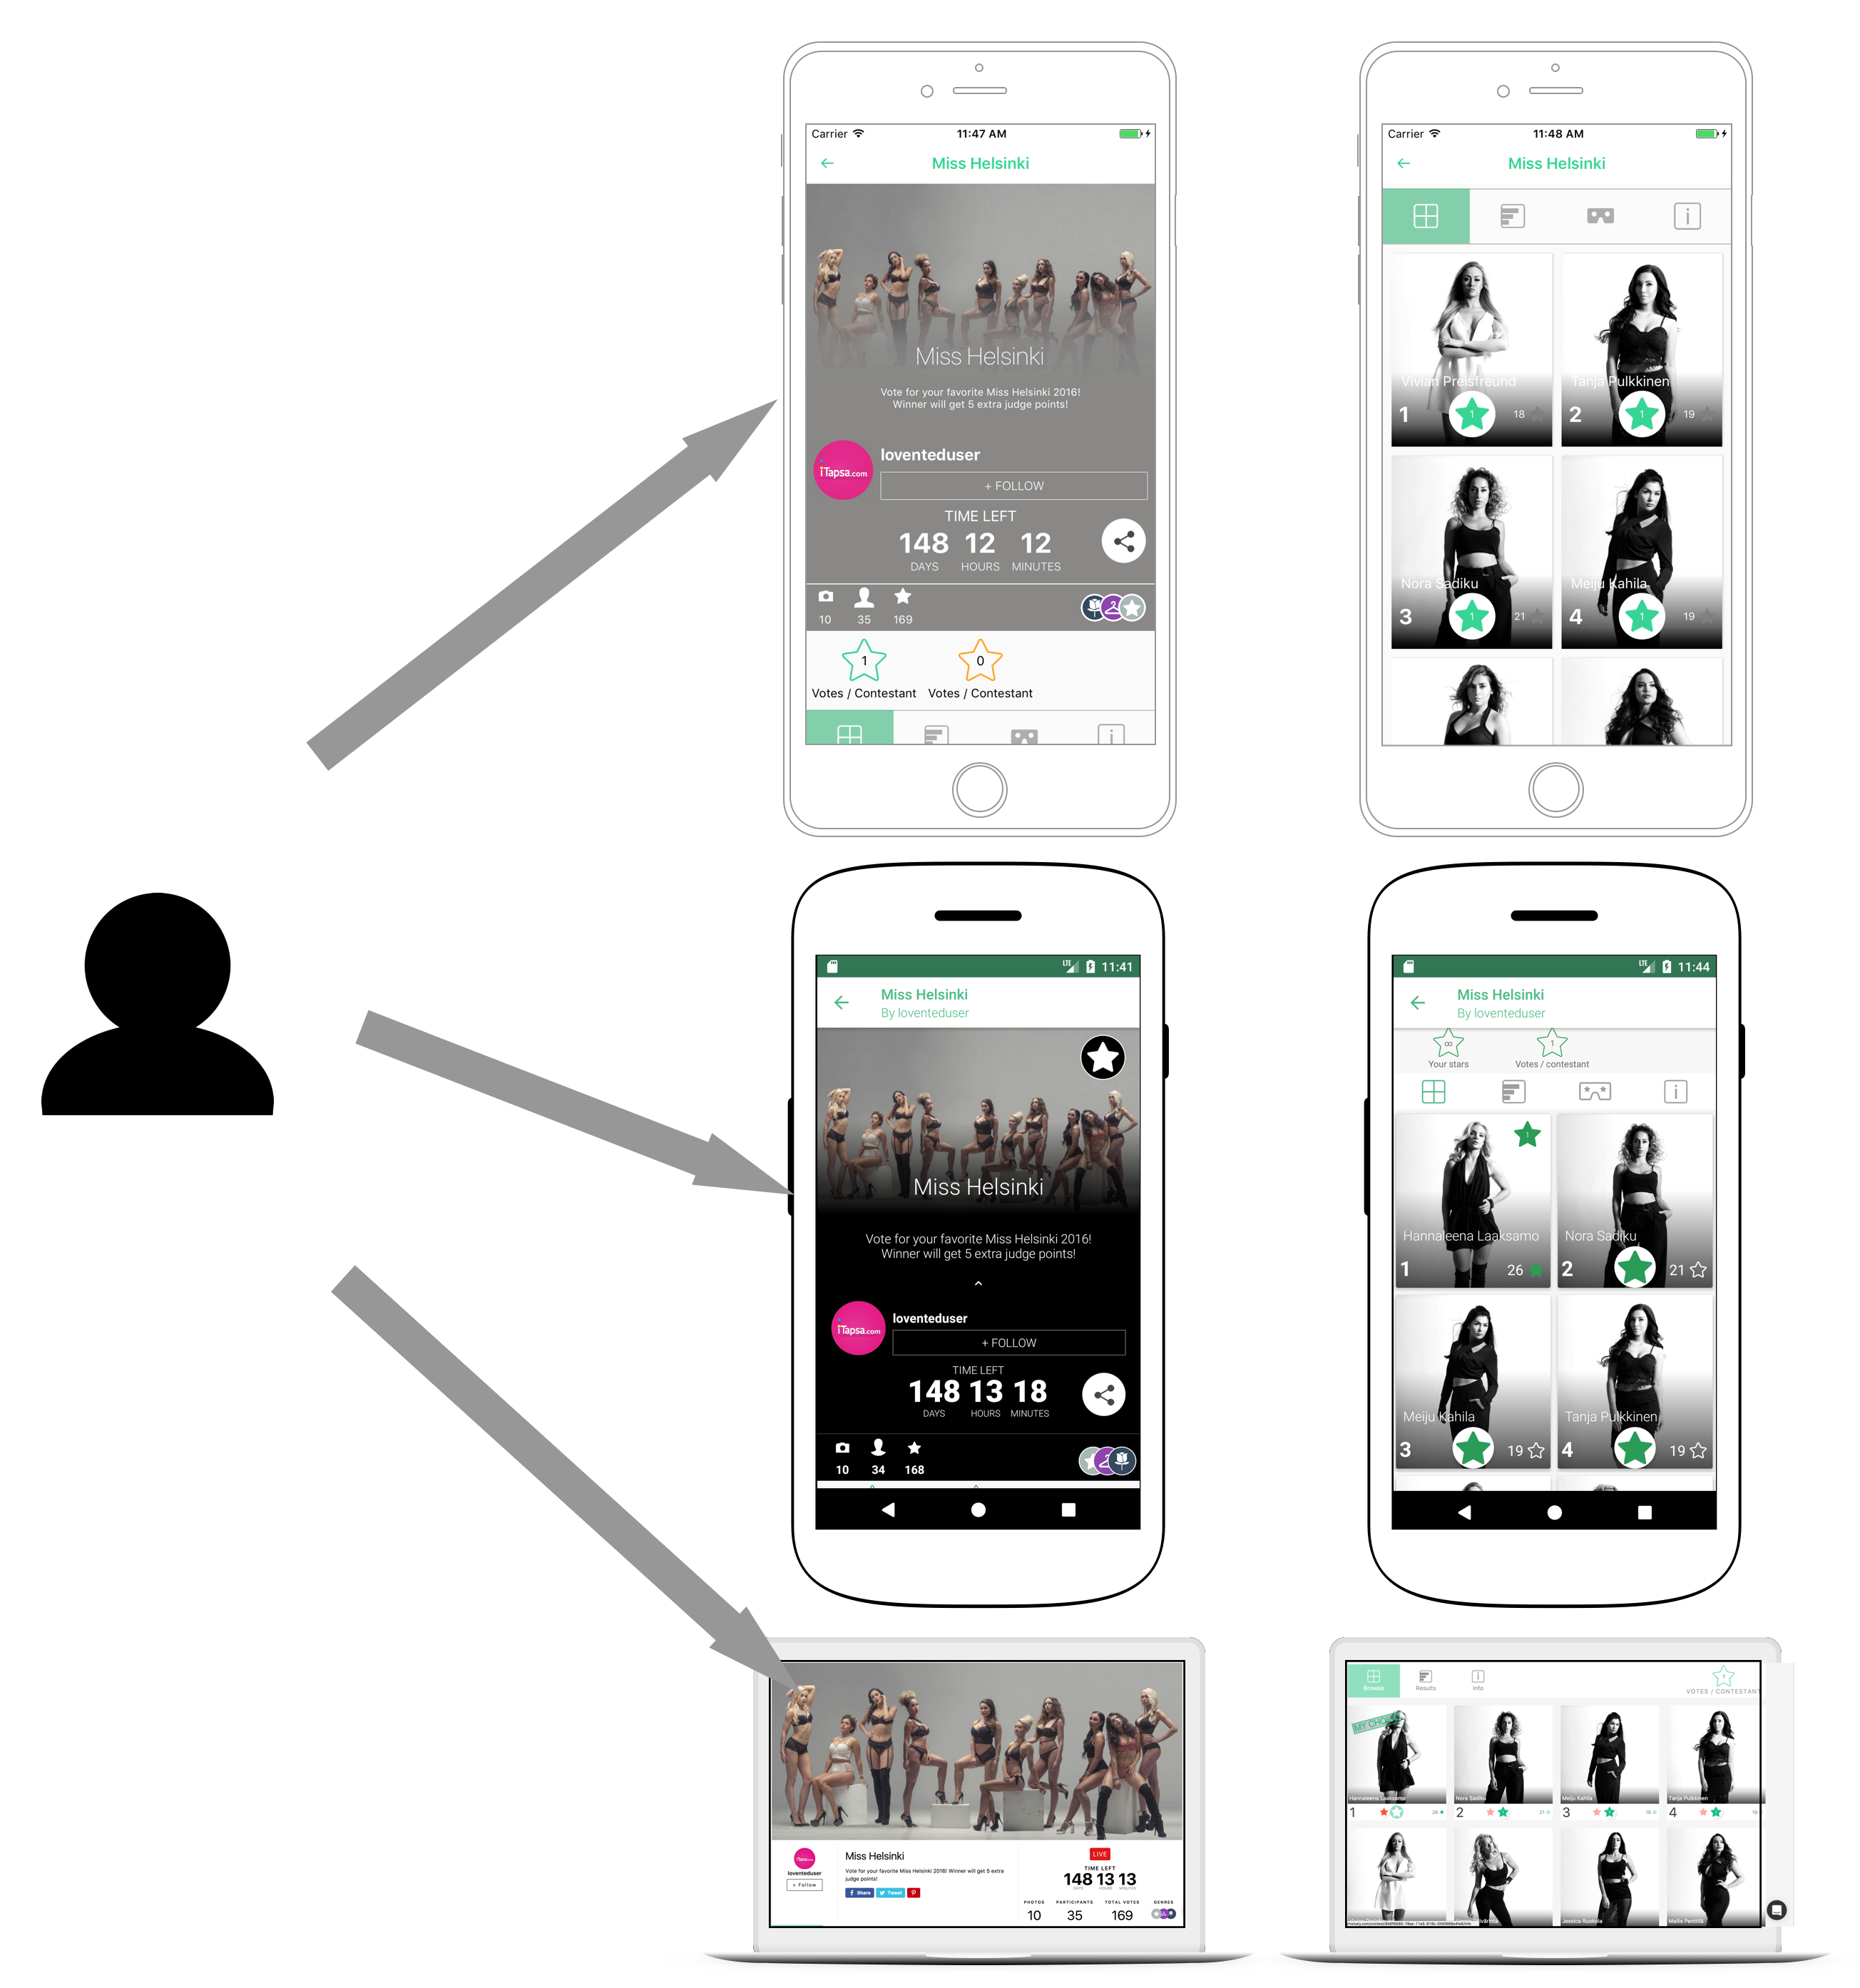
\includegraphics[width=0.6\textwidth]{images/choicely_platforms.png}
            \caption{Users can vote in contests through three interfaces: iOS devices, Android devices and web.}
            \label{choicely_platforms}
        \end{center}
    \end{figure}

    % what do users have to do to participate? 
    Majority of the contests require users to have a user profile in the Choicely platform. Choicely offers authentication through social media (Facebook and Google+) as a convenient option for users to sign up with one click. Optionally, user profiles can be created through a regular sign-up process, where users pick a username as their identities. When users choose this kind of registration, their e-mail addresses are confirmed through a verification link sent to their inbox, so that their identity is confirmed. Each user profile contains the features listed in Table \ref{user_profile_fields}. 

    \begin{table}[]
        \centering
        \begin{tabular}{l|l}
            \textbf{Field}              & \textbf{Type} \\
            \hline
            Full name                   & Free text \\
            Profile picture             & Image \\ 
            Cover image                 & Image \\
            Gender                      & Male/Female/Other/Not specified \\
            Location                    & Country, state and city \\
            Birthday                    & Datetime \\ 
            Age group                   & 0-17/18-24/25-34/35-44/45-54/55-64/65+ \\
            Introduction/Bio            & Free text
        \end{tabular}
        \caption{The list of fields and their types for each user profile.}
        \label{user_profile_fields}
    \end{table}

    % other contest-related data
    Contests also have some meta data which can facilitate data analysis. Each contest belongs to at least one but up to three of the following categories: animals, beauty, danger, design, entertainment, fashion, food, games, humor, sports, travel, other. The category labels are aligned by the contest's author upon creation. Contests also have starting and an ending time, between which users can vote or participate in them. While votes arrive into a contest, the vote count value tells the number of total votes received, while the number of unique voters tells how many individual users have voted in the contest.   

    % what kind of data is generated?
    Consequently, the available data is two-folded: the user profiles contain demographic information about the users (age group, gender and location), while contests have a number of participants with arbitrary number of votes that the users have spent on them. The latter kind of data can be seen as digital footprints generated by users in the Choicely platform. The combination of these datasets sums up to the user data as explained in the previous chapter and Figure \ref{user_data_venn} in this particular case. This is further supported with the meta data of contests explained in the previous paragraph. 

    %The vote changes for the contests are stored as transactions. This means that the database contains not the final results of the voting, but rather the changes what users made while using the software. This way it is possible to analyze the votes over time and to look at changes individually. For instance, it is possible to tell if a user has removed his/her votes from participant A and moved them to participant B. Furthermore, this way of data representation to restore or simulate any previous state of the contest, in case it would be needed.

\subsection{Research setting}
    % why is the data analysis relevant from scientific research point of view?
    Performing scientific research on such data is interesting for multiple reasons. To begin with, at the time of this research Choicely does not utilize data analysis tools to gain better understanding on the collected data. It is in the interest of the company and its customers to better understand what kind of audience was engaged in the past, what kind of content is more (or less) successful and what tendencies in user behavior can be extracted from the data. As a result, the introduction of data analysis and visualization tools at the company will greatly enhance business value of the firm, provide deeper understanding on the domain as well as the existing user base.   
    
    % how is Choicely different than other social networks or any other repository of user data?
    Secondly, Choicely can be looked at as a social network, because some of the platform uploaded to the platform is generated by users. Users also have the possibility to express their appreciation or support towards some contest participants by spending votes on them. Similarly to social networking sites, where the "like" feature is often used \cite{jang2015noreciprocity, bakhshi2014faces} this phenomena can be looked at as a way of expressing personal opinion. 
    
    In comparison to most of the currently available social networks, voting platforms like Choicely are observed by the audience differently. On one hand, social media sites usually list posts or images on a feed, where there is theoretically no relation between the posts that follow eachother. On the other hand, contestants in the Choicely platform share similarities as they were nominated for the same contest. Accordingly, there must be some similarity among them as all are subjects of the contest's topic, rules and are competing for the best possible result. 

    % so what? Why is that important from user point of view
    This slight difference in the content makes a big change in terms of user behavior. The focus moves from "what kind of content I like" to "which piece of content I like the most in comparison to the rest". Consequently, users will scan through some (or optimally all) of the contestants and make unconscious decisions upon whether to give vote(s) on certain contest participant(s). The users express their favour and support towards a subset of contenders, and hence helping them to reach their ultimate goal: winning in the contest. 
    % how can this contribute to user behavior and social media studies? 
    This difference compared to other social networking sites offers a great possibility for research. The potential of identifying what kind of content among different contests individuals like as well as what kind of content similar group of users like, hinders in the data.    

    % how computer vision is going to be utilized? 
    One of the challenges in connecting users with topics of contests is that there is no indication on what the content on the contenders' pictures is. Contest authors only assign categories to the contests to be created, which does not necessarily describe the entrants in the contest. Other researches have successfully utilized computer vision to gather meta data for the uploaded content in image sharing communities \cite{bakhshi2014faces, hu2014we}. 
    
    % what is the solution to this problem?
    Deriving from the success in previous studies \cite{hu2014we, farseev2015harvestingmultiplesources, han2016teensarefrommars, bakhshi2014faces}, computer vision is utilized in this research to identify labels that appear on the participants' images. For instance, a beauty pageant's entry image may be labelled with meta data, such as "Beauty", "Photo Shoot", "Smile" and "Blonde". Similarly, a design contests entry might have topic labels, such as "Landmark" or "Architecture". Figure \ref{google_vision_labels} displays an example, where the Google Vision API was used to extract such labels from images, that were participants in two of Choicely's contests.

    \begin{figure}[h] 
		\begin{center}
            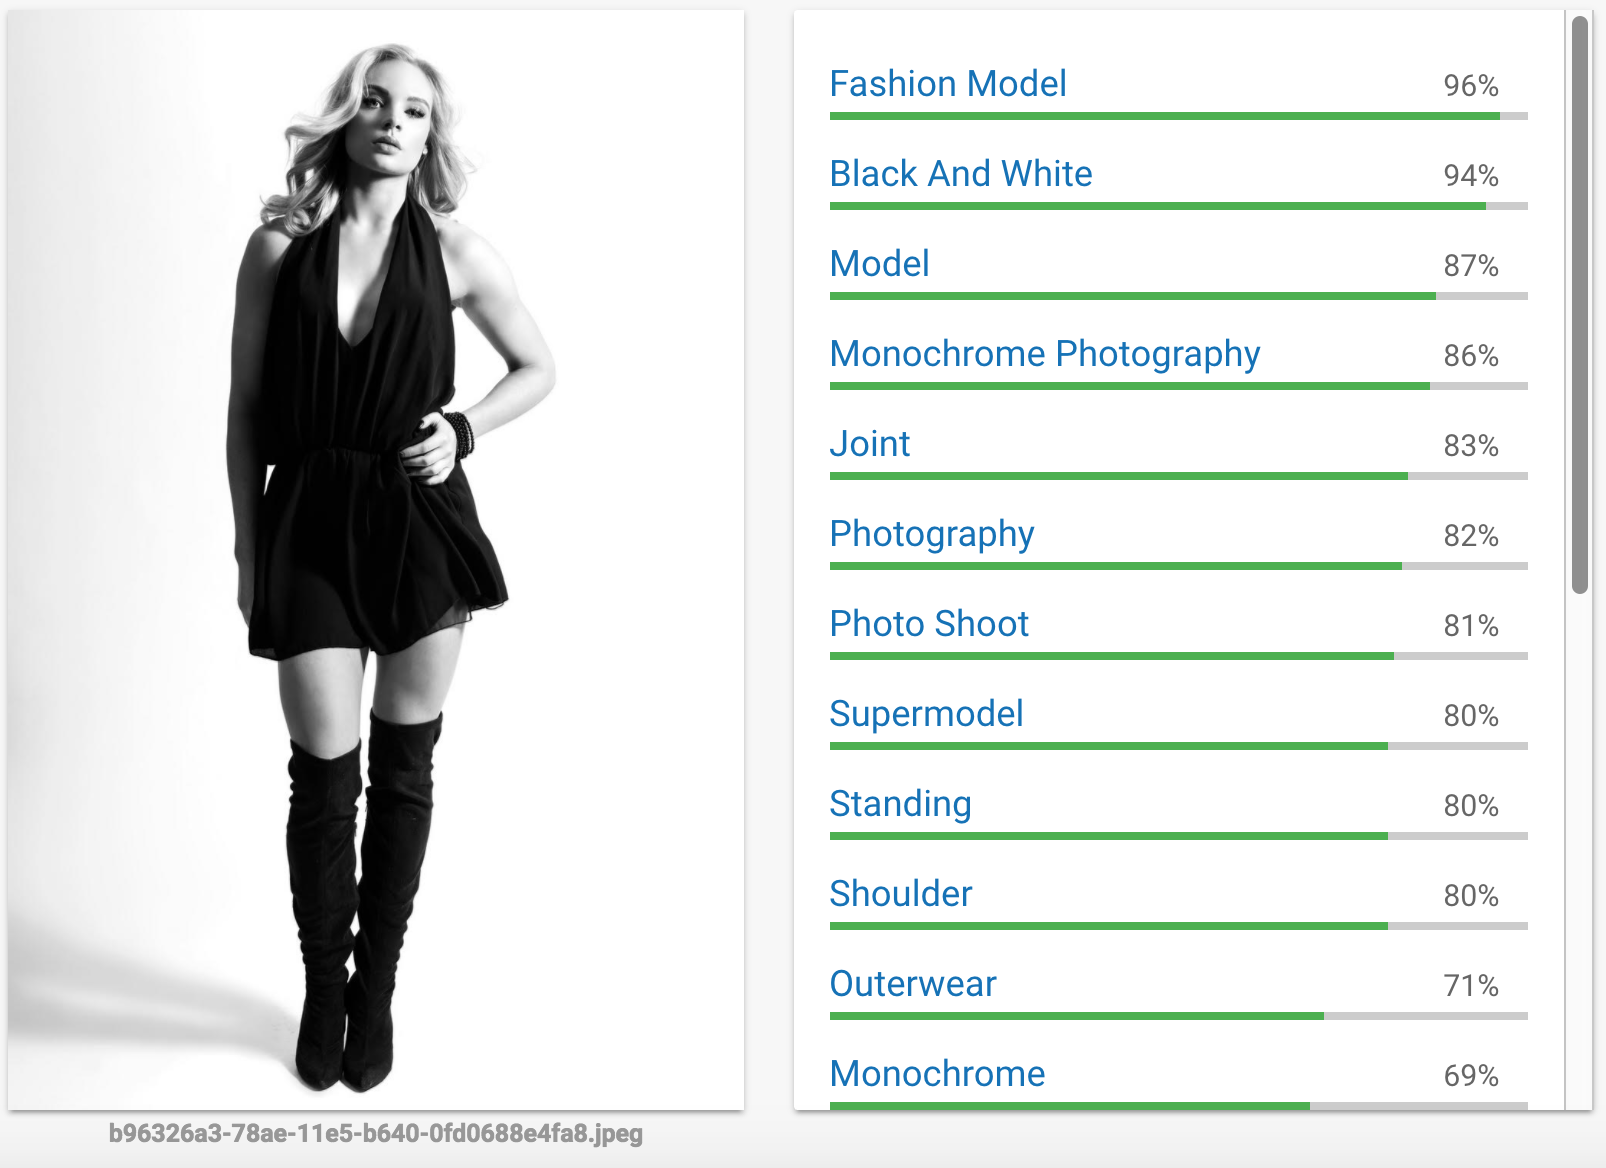
\includegraphics[width=0.8\textwidth]{images/google_vision_labels.png}
            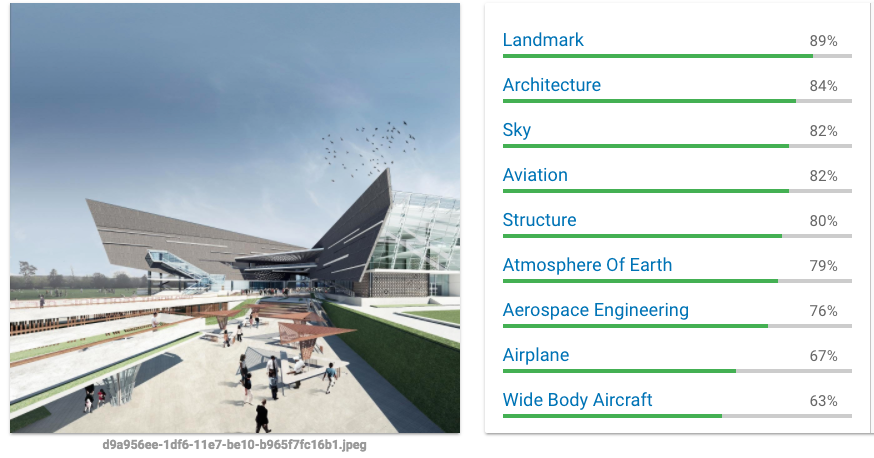
\includegraphics[width=0.8\textwidth]{images/google_vision_labels2.png}
			\caption{The labels identified by the Google Vision API on two of the contest participant's images.}
			\label{google_vision_labels}
		\end{center}
    \end{figure}

    % how are the labels used - what is the method performed on them? 
    Combining the identified labels and the vote data can provide information on user behavior. For instance it can be identified which demographic group of users like what kind of content, or the behavioral differences between two or more groups can be compared to eachother. Furthermore, this kind of information could be used to recommend new content in the platform to users which they have not seen before. Last but not least, it could be identified that which traits of participants contribute to more votes and engagement by users or certain user groups.  
    
    \subsection{Data structure}
    % architectural overview
    The current architecture of the Choicely platform is...
    \begin{figure}[h] 
		\begin{center}
            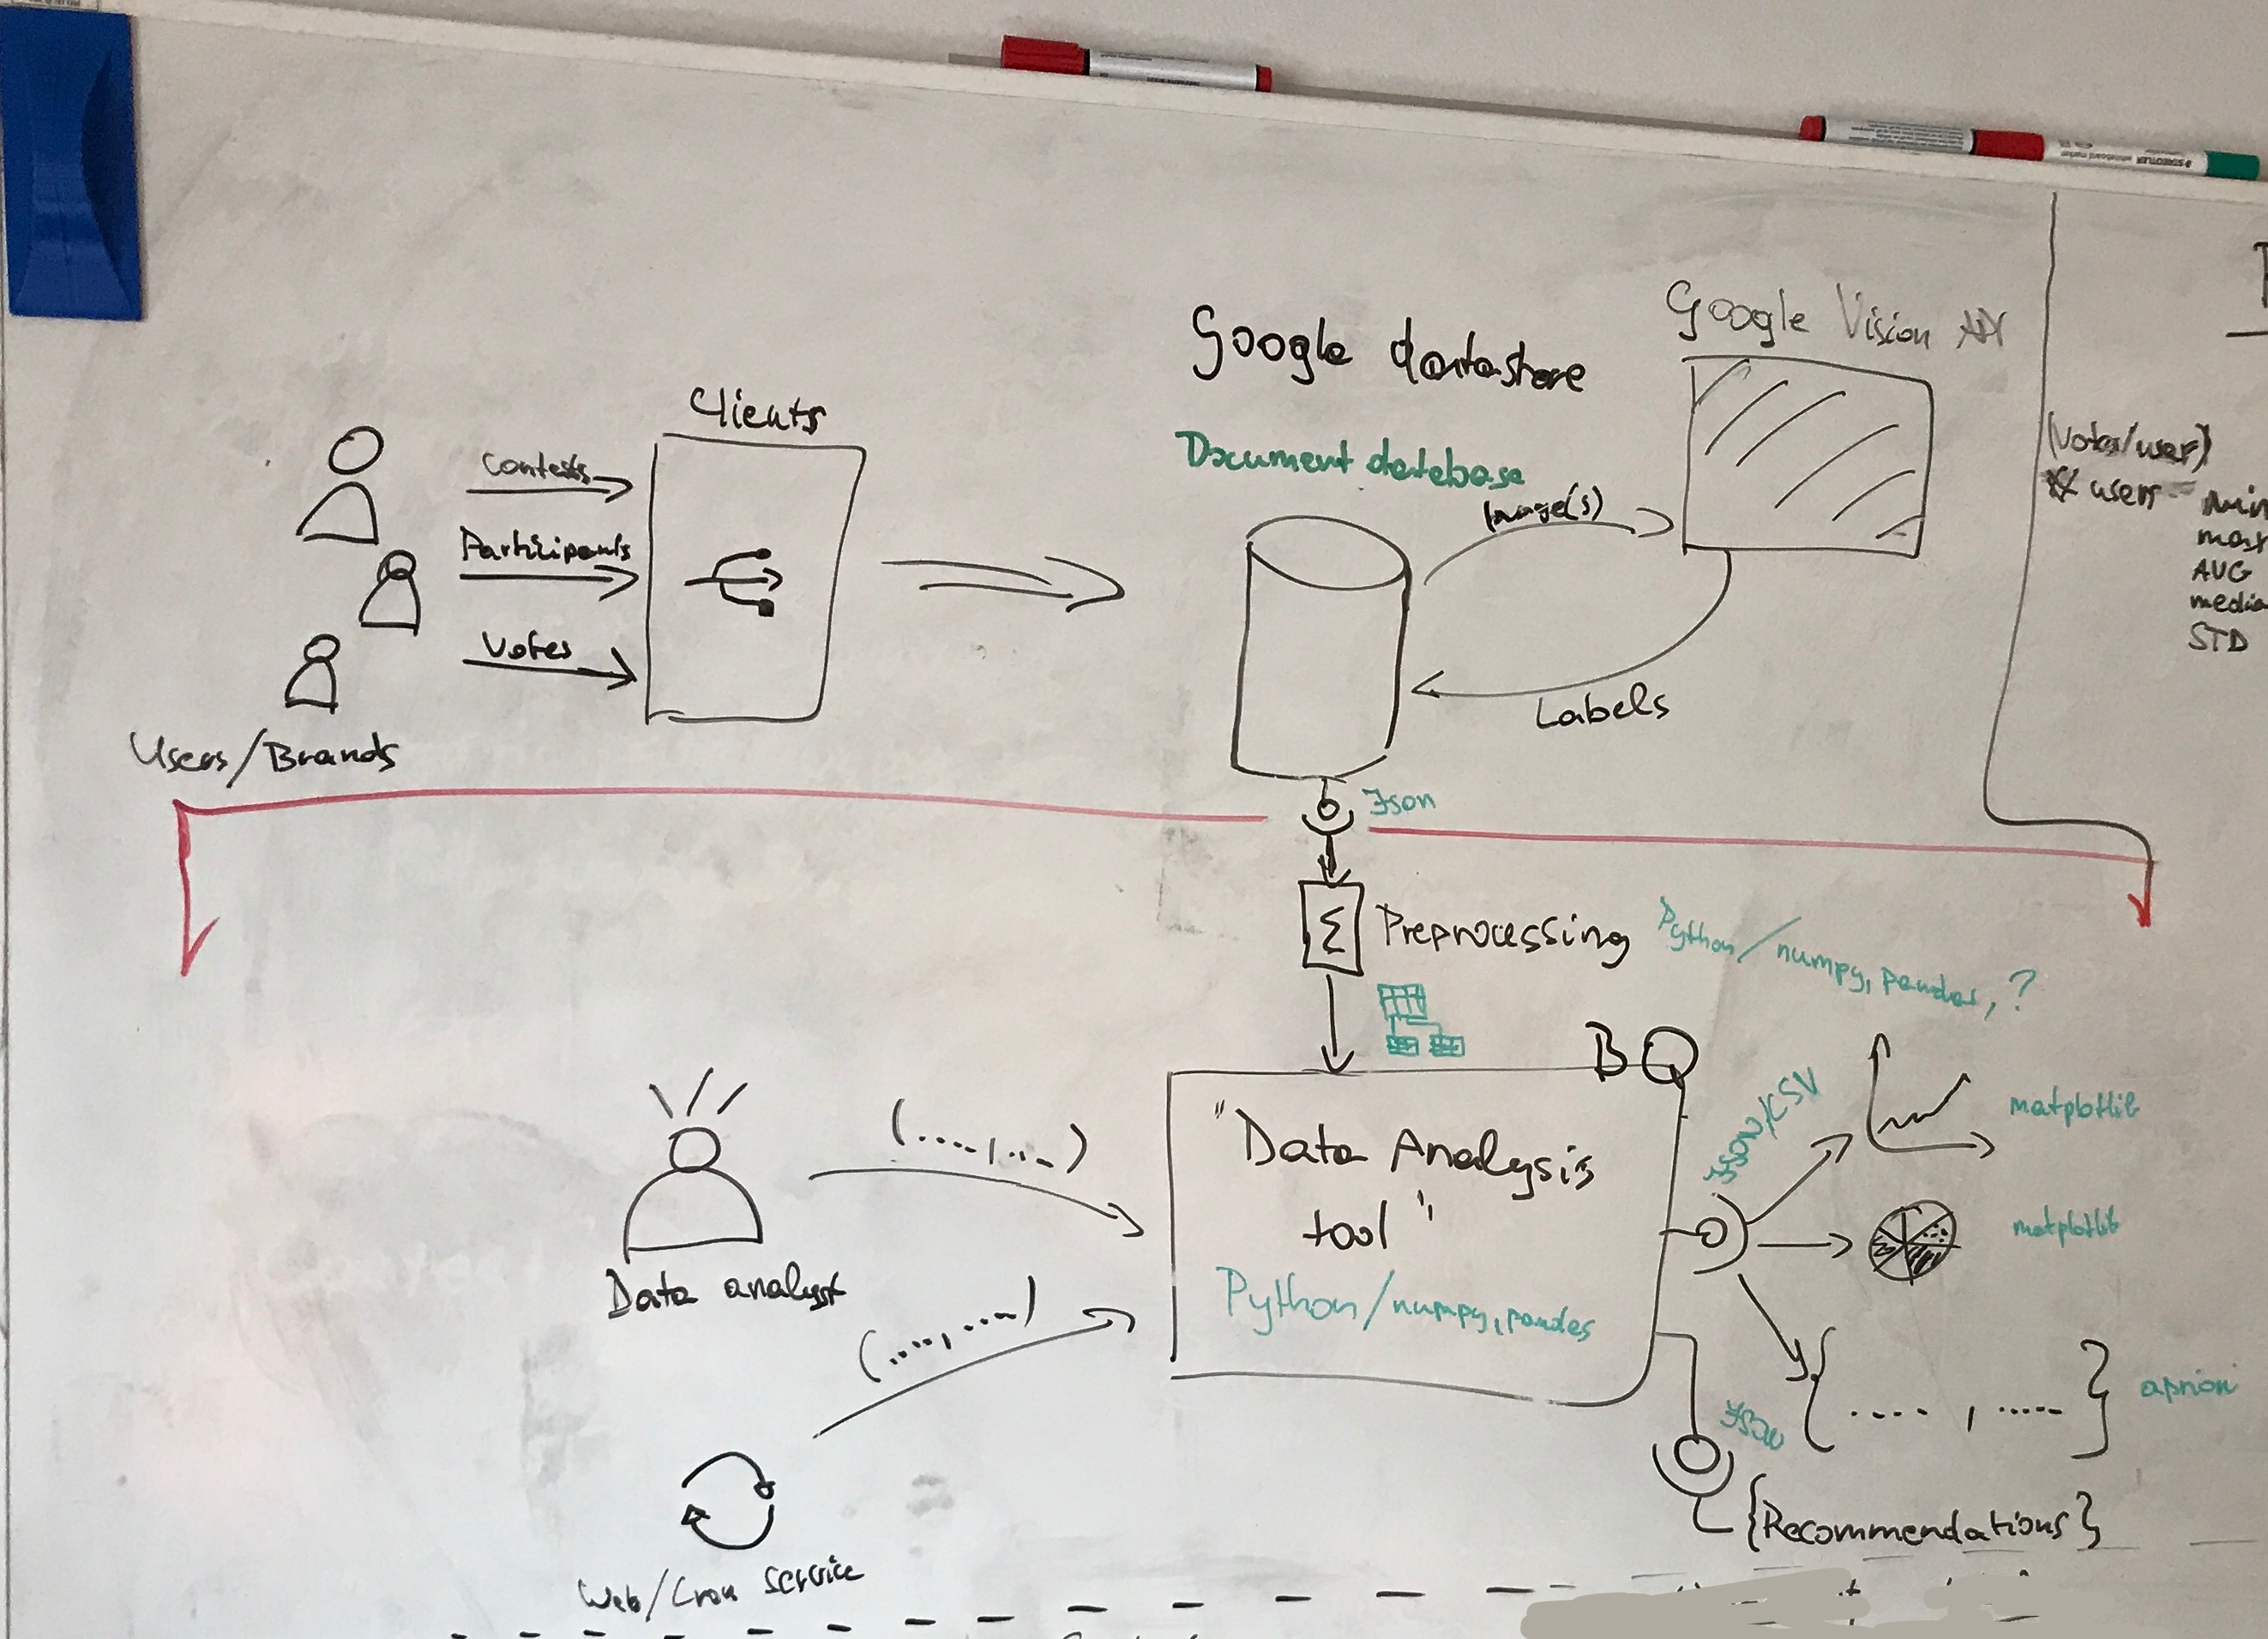
\includegraphics[width=0.8\textwidth]{Images/architecture_whiteboard.jpg}
			\caption{The brief architectural overview of the Choicely platform.}
			\label{choicely_architecture}
		\end{center}
    \end{figure}

    \begin{figure}[h] 
		\begin{center}
            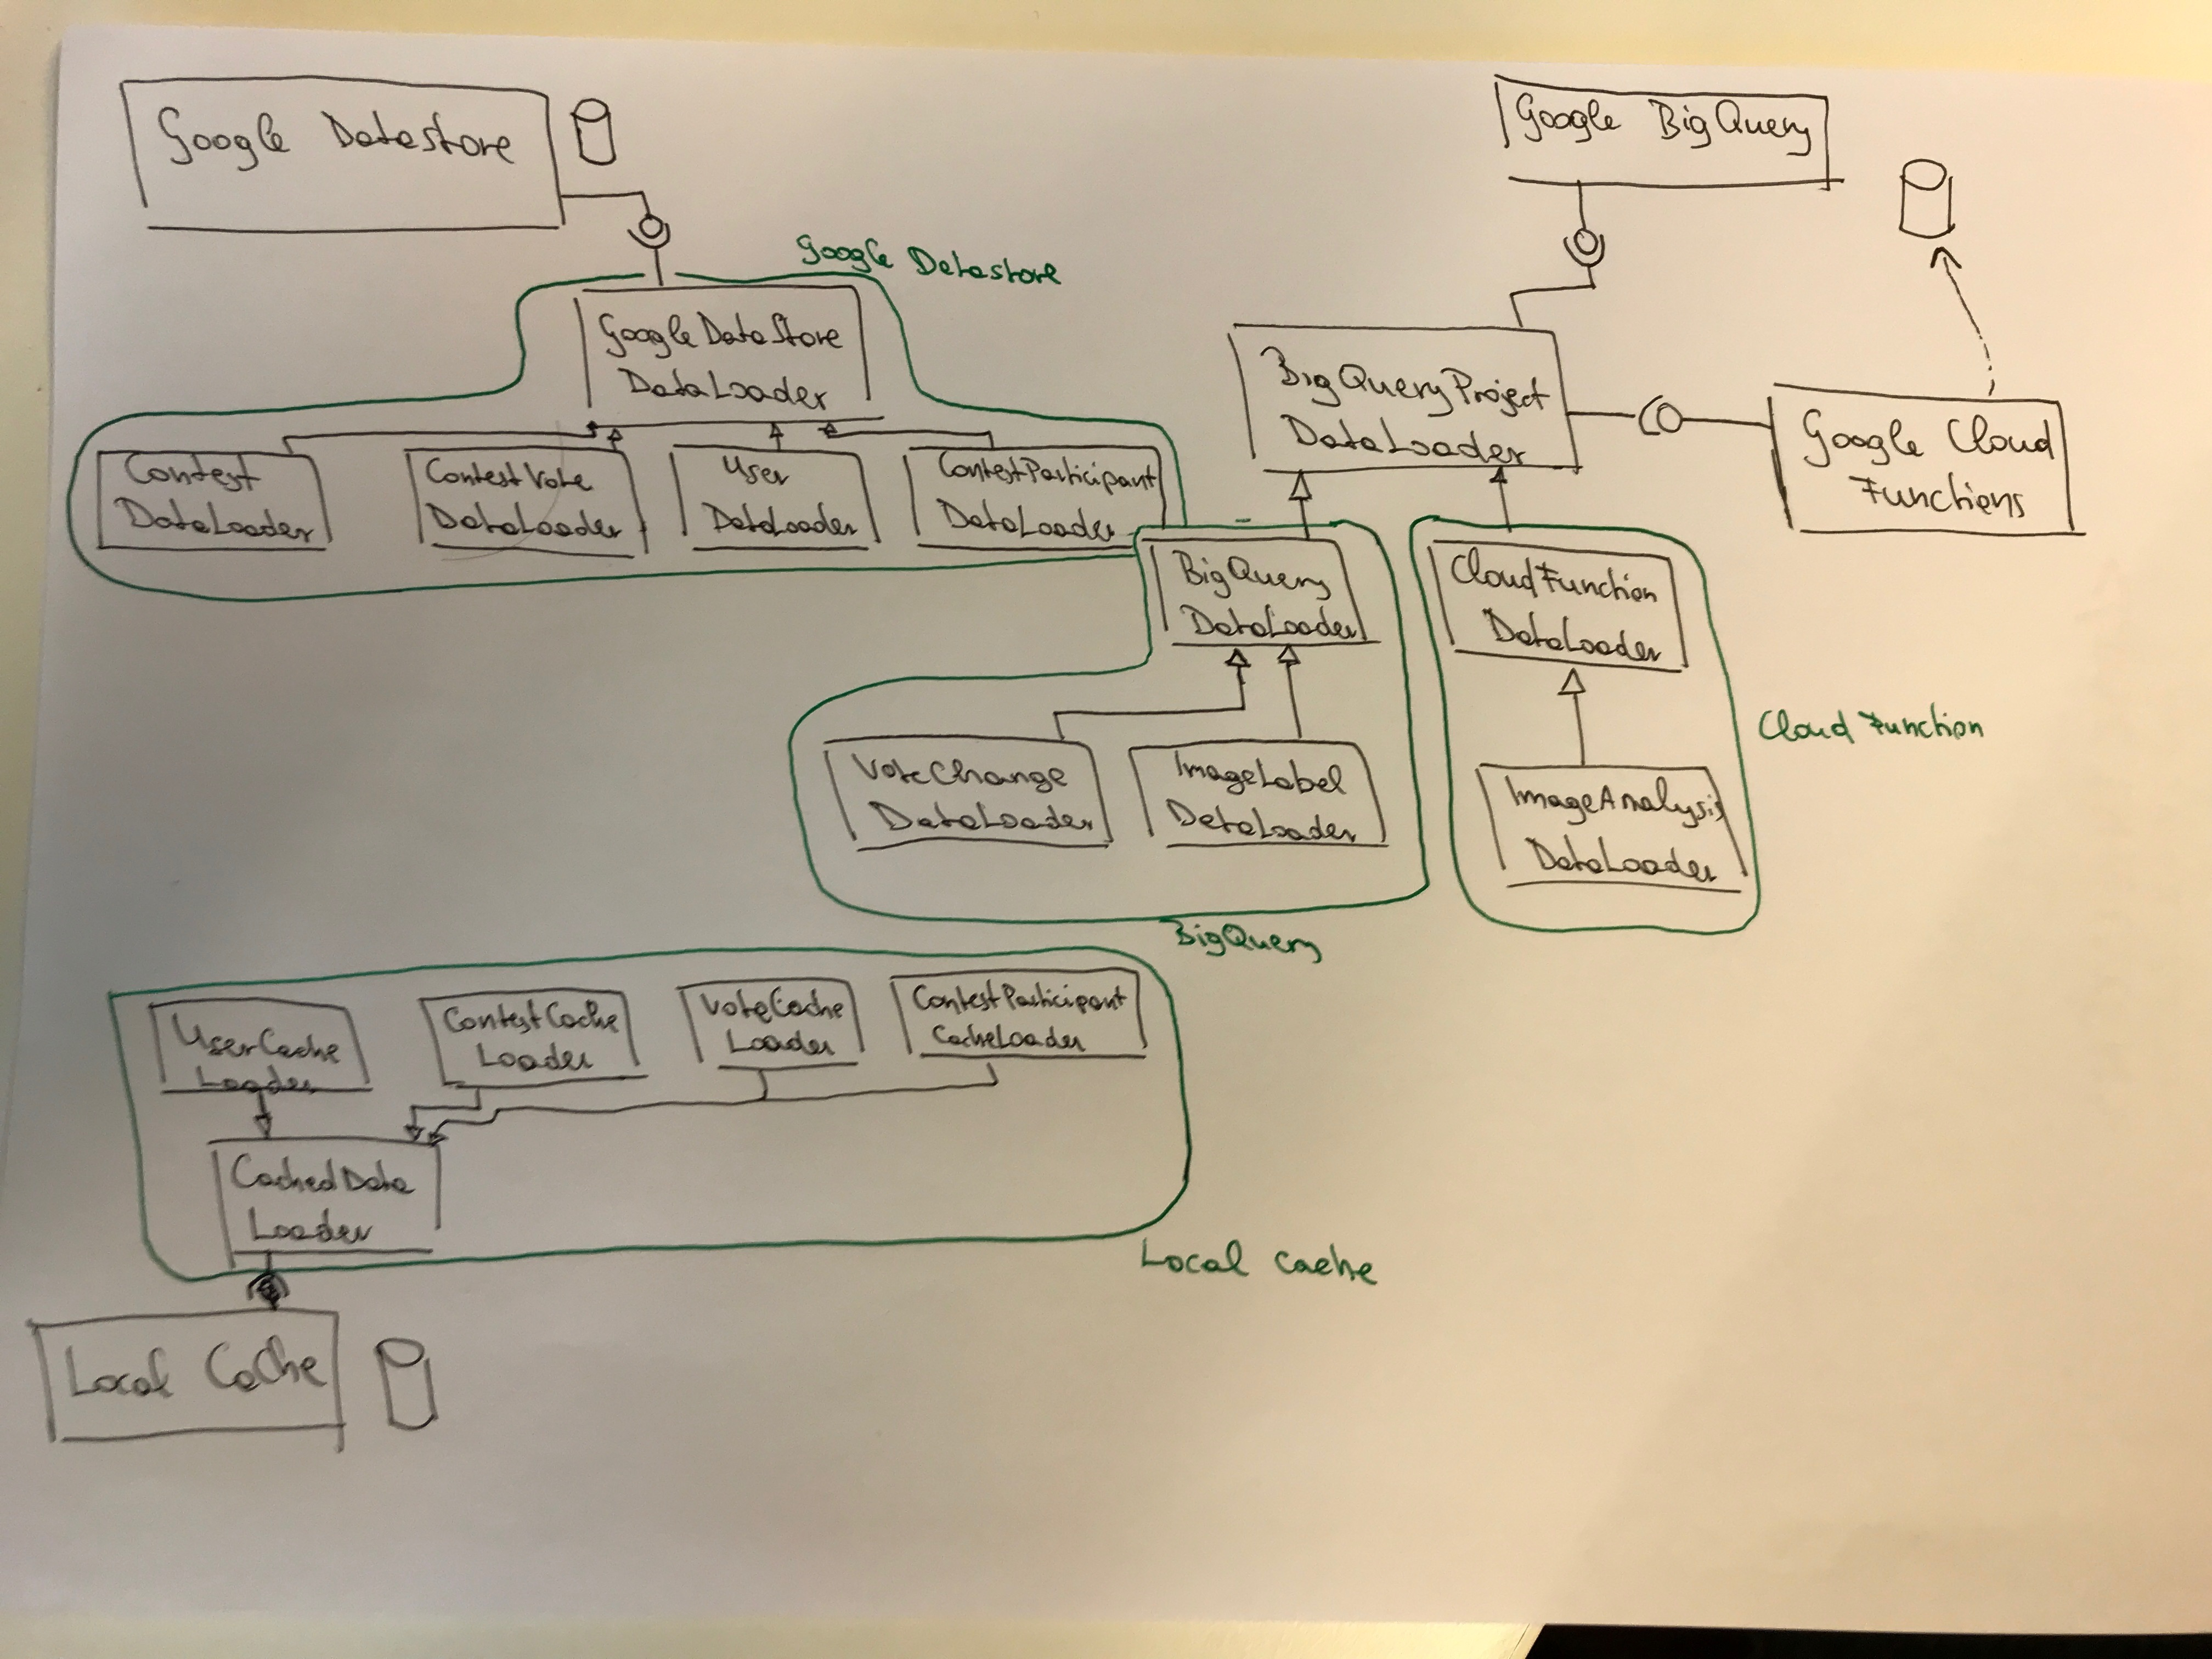
\includegraphics[width=0.8\textwidth]{Images/IMG_1317.jpg}
			\caption{The data sources of the data analysis in the Choicely platform.}
			\label{choicely_data_sources}
		\end{center}
    \end{figure}

    % the structure of the data models
    The structure of the data... 
    \begin{figure}[h] 
		\begin{center}
            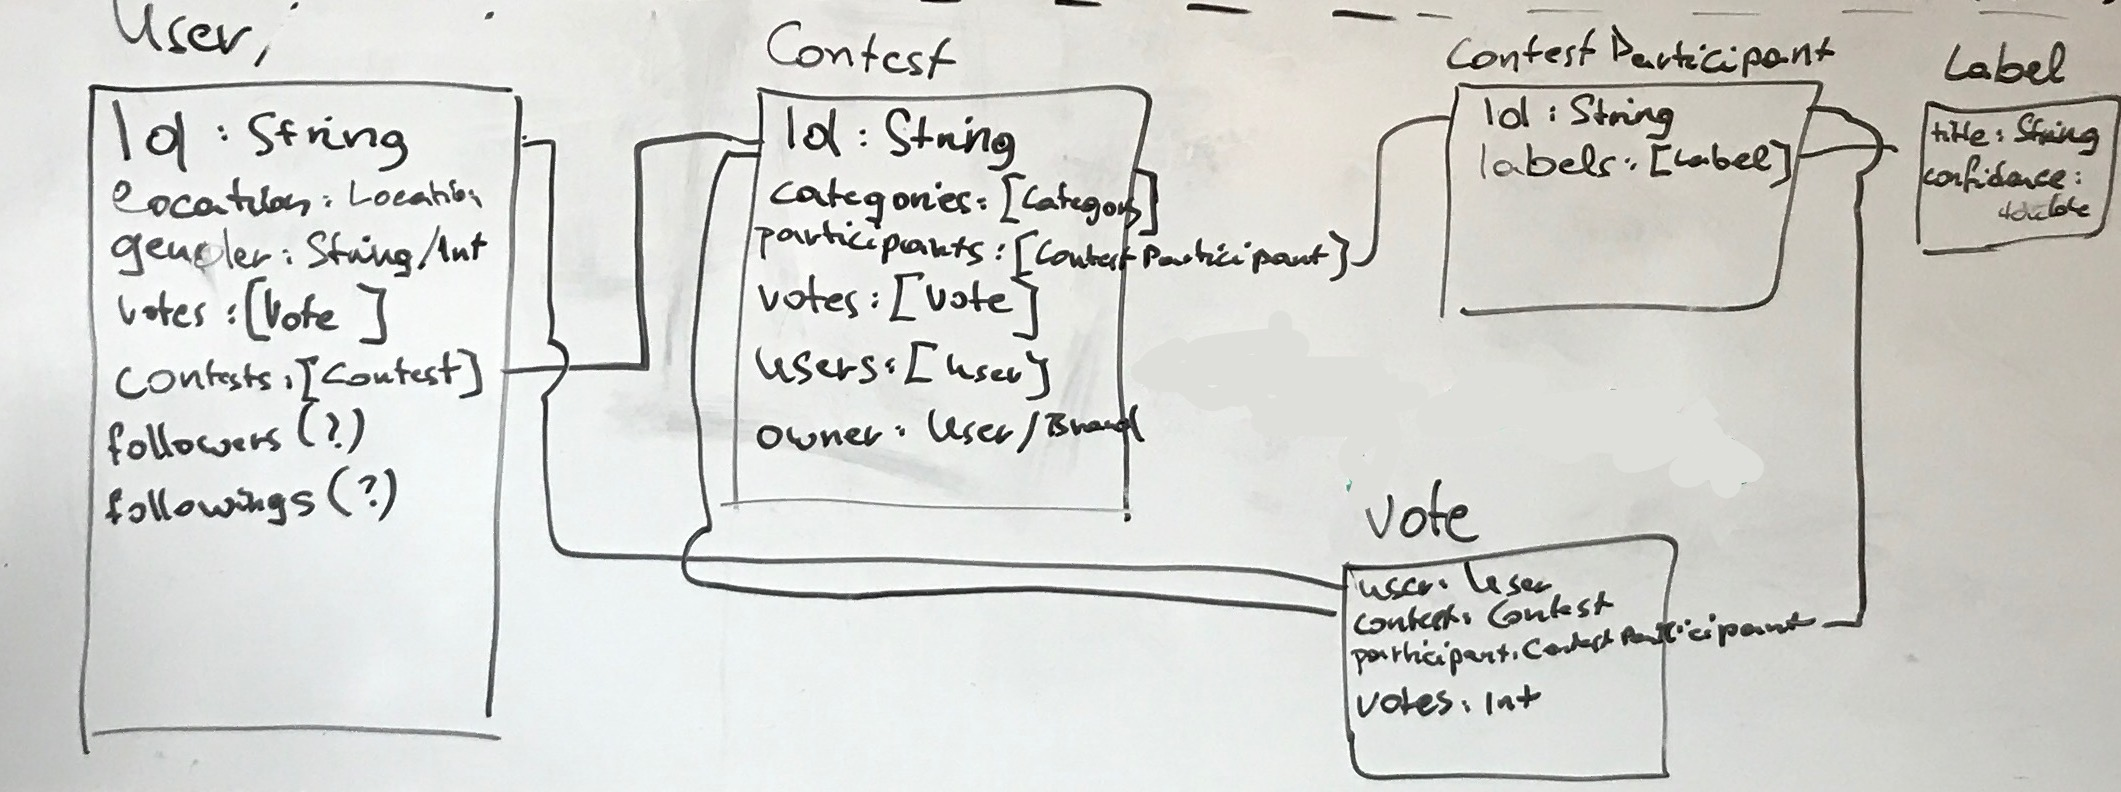
\includegraphics[width=0.8\textwidth]{Images/data_structure_whiteboard.jpg}
			\caption{The structure of the data models of the Choicely platform.}
			\label{choicely_data_models}
		\end{center}
    \end{figure}

\subsection{Methodology} % what kind of methods were chosen? 
    % Exploratory Data Analysis (EDA)
    To grasp on the currently available data, Exploratory Data Analysis (EDA) is utilized as the first step of the research. A comprehensive overview on the data related to the most important entities in the Choicely platform is performed by calculating basic statistical measures and visualizing the data. Such entities are the user profiles, the contests, contest participant and the votes performed by users on the contest participants. The findings of the EDA are then utilized to determine how to prune the data such that the acquired sample is representative, does not contain redundant nor faulty data. The results of the EDA are explained in the next section. 

    % Preprocessing and pruning
    Based on the results from the EDA, a subset of contests is chosen for more careful analysis. The subset of the contests is limited to those, which have engaged the most users and gathered a higher enough number of votes and unique voters (users who have voted at least once in the contest). After applying the pruning rules, some part of the data is preprocessed so that the analyses can be performed easily. The pruning rules and preprocessing steps are explained in the next section. 

    % Association Analysis
    Finally, Association Analysis is performed on the combined demographic, vote and the image label data in the chosen contests. The list of labels extracted from the participants in the contest are listed for each of the voters' transactions alongside with the voters' demographic data. The data retrieved from the three sources is combined as shown in Table \ref{association_analyisis_data}. Frequent Itemset Analysis is then performed on the data to identify behaviors and preferences of the different demographic groups. Association Rule Discovery is performed on the same data to understand which pair of traits can engage more of the (targeted) audience.  

    \begin{table}[]
        \centering
        \begin{tabular}{l|l|l|l|l}
            gender & age group & country & image id & labels \\
            \hline
            female & 25-34 & fin & 9d33085c-... & ['fashion model', 'hair', 'model', 'beauty', '...] \\
            female & 18-24 & fin & 9d33085c-... & ['fashion model', 'hair', 'model', 'beauty', '...] \\
            female & 65+ & fin & 9d33085c-... & ['fashion model', 'hair', 'model', 'beauty', '...] \\
            female & 18-24 & swe & 9d33085c-... & ['fashion model', 'hair', 'model', 'beauty', ...] \\
            female & 18-24 & swe & 9d134a94-... & ['beauty', 'blond', 'human hair color', 'model', ...]
        \end{tabular}
        \caption{The format of the data used for Association Analysis.}
        \label{association_analyisis_data}
    \end{table}

    % check \cite{socialdiversityongithub} -> Blau index / diversity index: reflects how many different types (such as species) there are in a dataset (a community), and simultaneously takes into account how evenly the basic entities (such as individuals) are distributed among those types.
    
    % what are the decisions behind the choices? 
    % what were the alternatives and why were they rejected? 
    % performance comparison - why was the local cache added?

\subsection{Results}
    \subsubsection{Exploratory Data Analysis}
    % what are the takeaways of the EDA? 
    The EDA fundamentally focused on two aspects of the data at hand: the user engagement in contests and the completeness of user profiles. First, the findings related to the content, then the user profiles in the Choicely platform are presented in the paragraphs to follow.
    
    % content
        % unique voters
        At the time of conducting this research, there is a total number of 536 contests in the platform. All if the contests have a few attributes which can help answering RQ2 presented in the Introduction chapter. To gain an understanding on how many users are typically engaged in contests, the number of unique voters is studied in comparison to the number of contests. Figure \ref{user_engagement_in_contests} displays a histogram and a boxplot of these measures. 
        
        \begin{figure}[h] 
            \begin{center}
                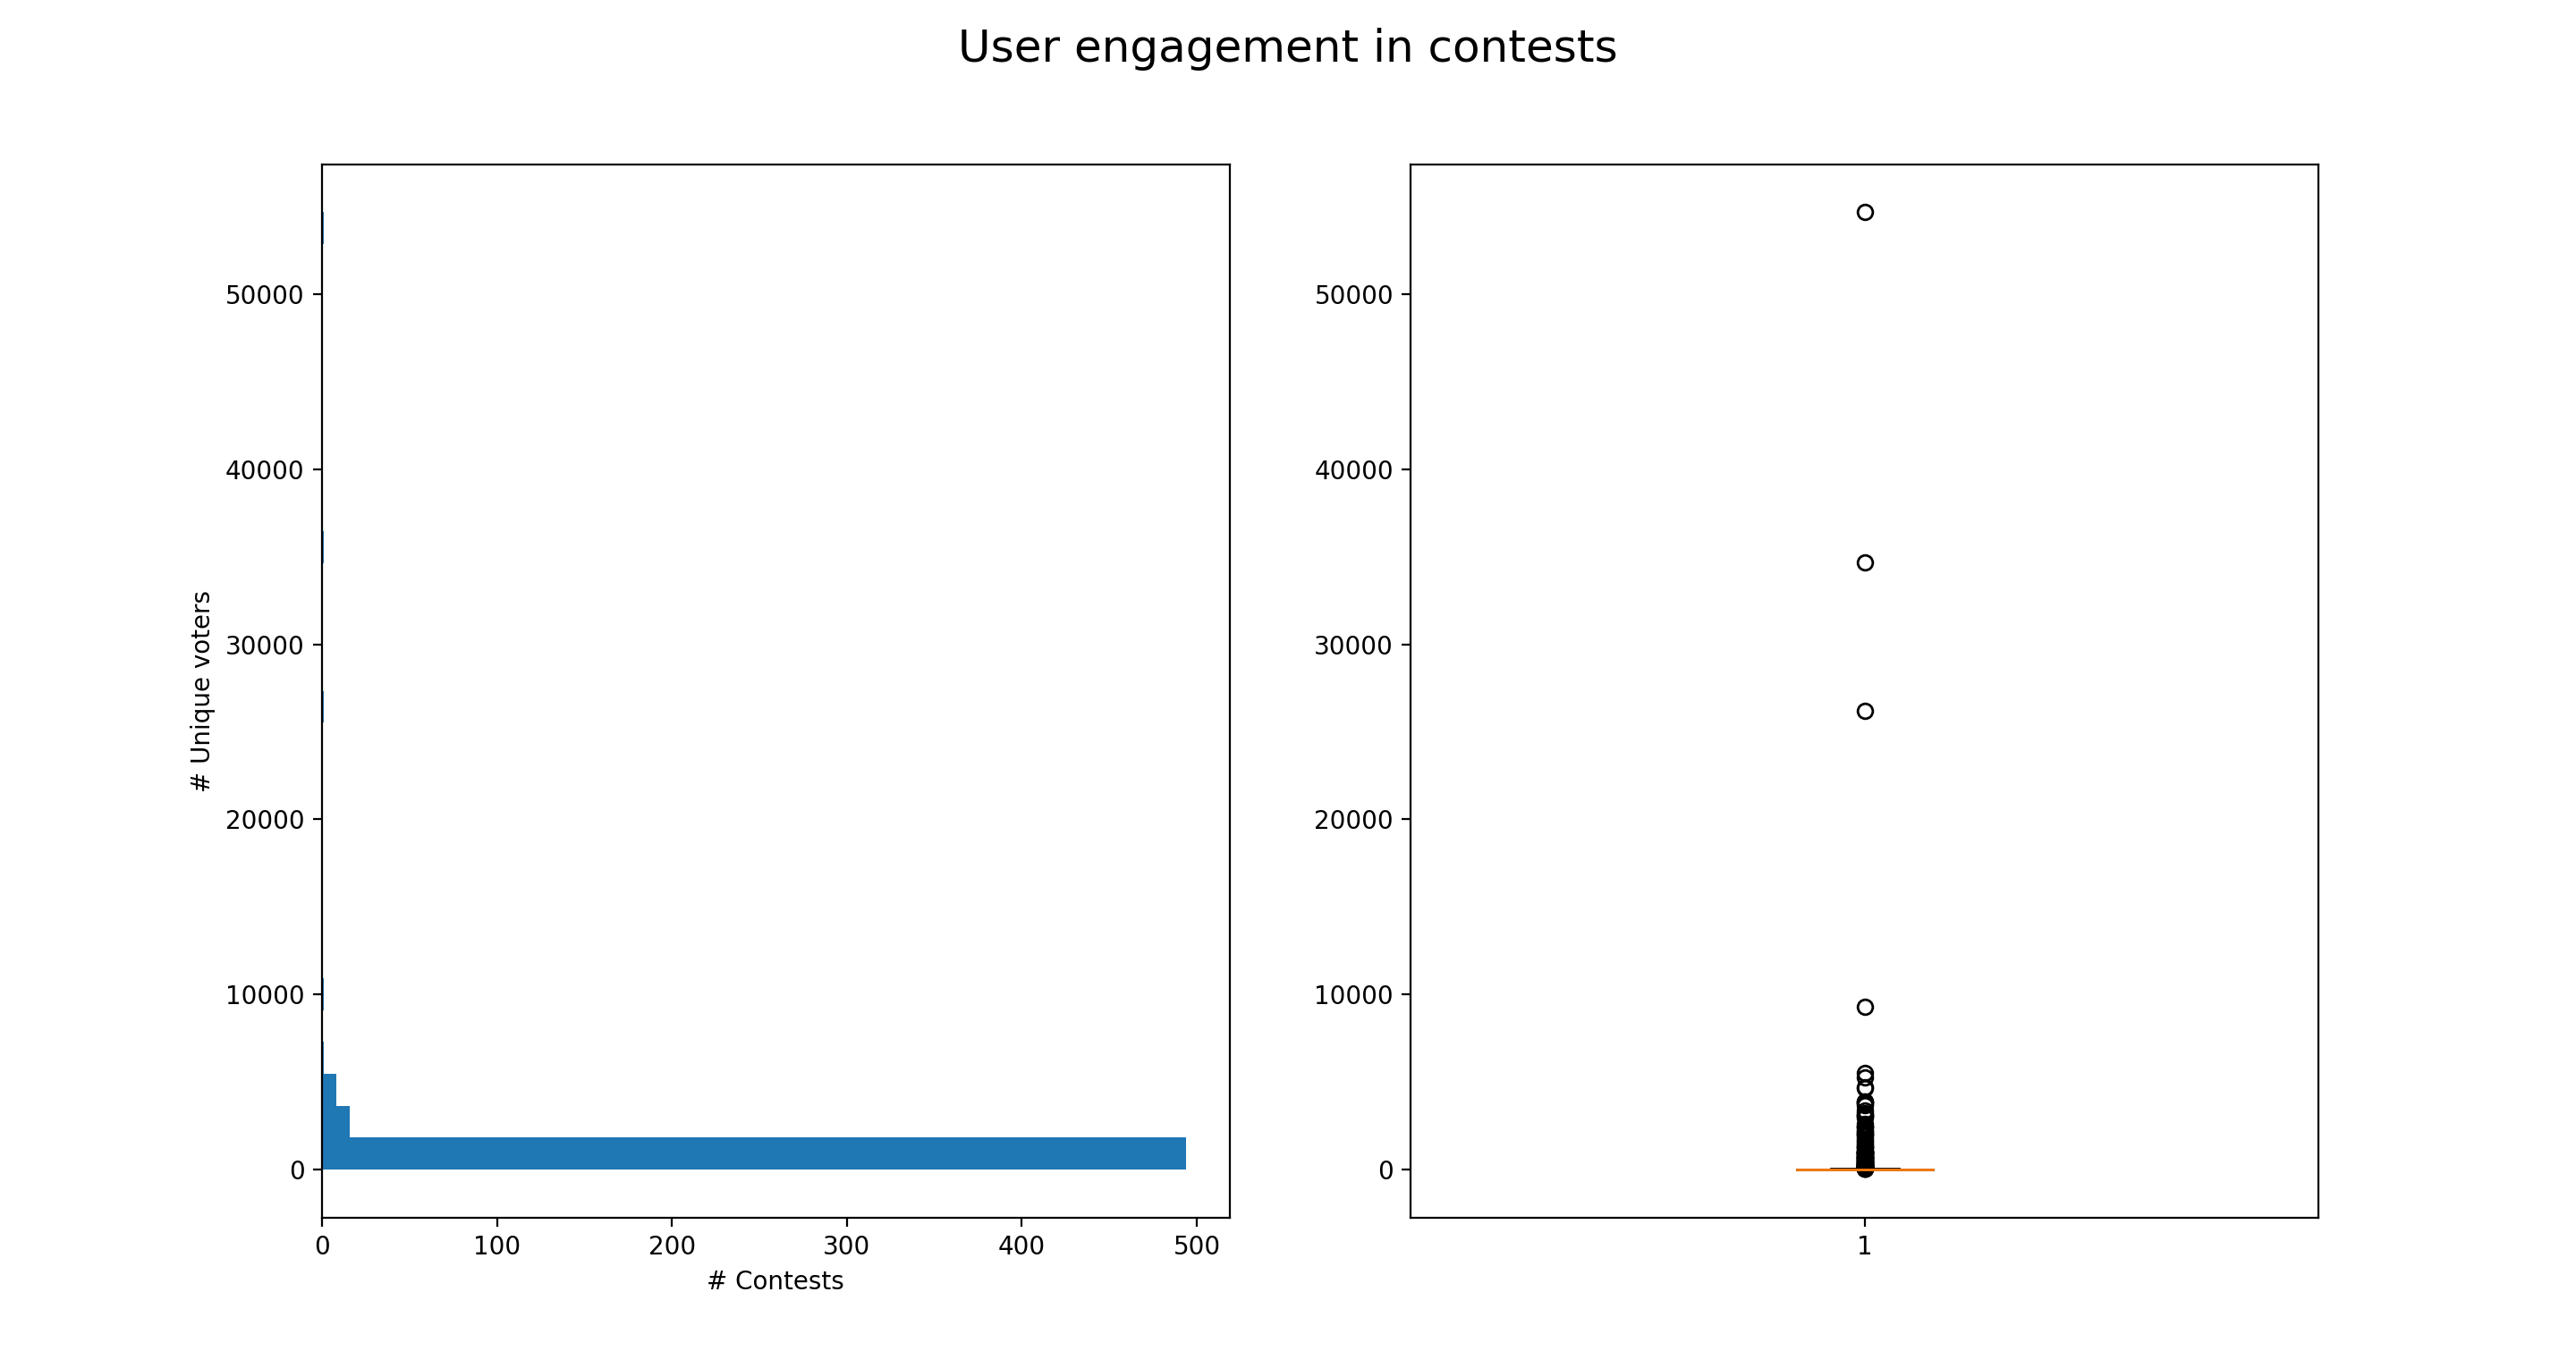
\includegraphics[width=0.8\textwidth]{Images/user_engagement_in_contests.png}
                \caption{The number of unique voters over contests.}
                \label{user_engagement_in_contests}
            \end{center}
        \end{figure}

        It can be easily seen that most of the contests engage very small amount of users, as the median of the unique voters value for all contests is 3. However, some of the contest have proven to be very successful, as the highest number of unique voters is close to $max_{unique_voters} \approx 55 000$. This observation is also supported with the mean value ($\mu = 464.65$) and the standard deviation ($\sigma = 3111.44$).These numbers allow us to conclude that many of the contests engage very small number of users. In order to retrieve a representative sample, contests with small enough unique voters is hence excluded in the pruning phase, which is explained in the next chapter. 
        
        Similarly to studying the number of unique voters on all contests, the same metric is broken down to all contest categories. The results are displayed on Figure \ref{user_engagement_in_categories}. It can be seen from the histogram, that a fairly high number of contests ($\approx 14 \% $) are categorized under the "other" category. This is probably due to the fact that authors did not assign the categories for one reason or another. It can be also seen that the amount of "beauty" and "fashion" contest is considerably high compared to the other categories, which is in align with the case company's profile at the point of conducting this study. From this visualization it is also visible that the amount of "sports" contests is considerably low ($\approx 3.5 \% $). After filtering out contests with only to the "other" category, it was identified that many of the sports, humor, design, beauty and fashion-related contests were indeed not labeled correctly in terms of their categories. This issue was fixed manually in the preprocessing phase. 

        % number of contests in overall, by category
        % explain the findings that there were too many "other" type of contests which were fixed manually
        \begin{figure}[h] 
            \begin{center}
                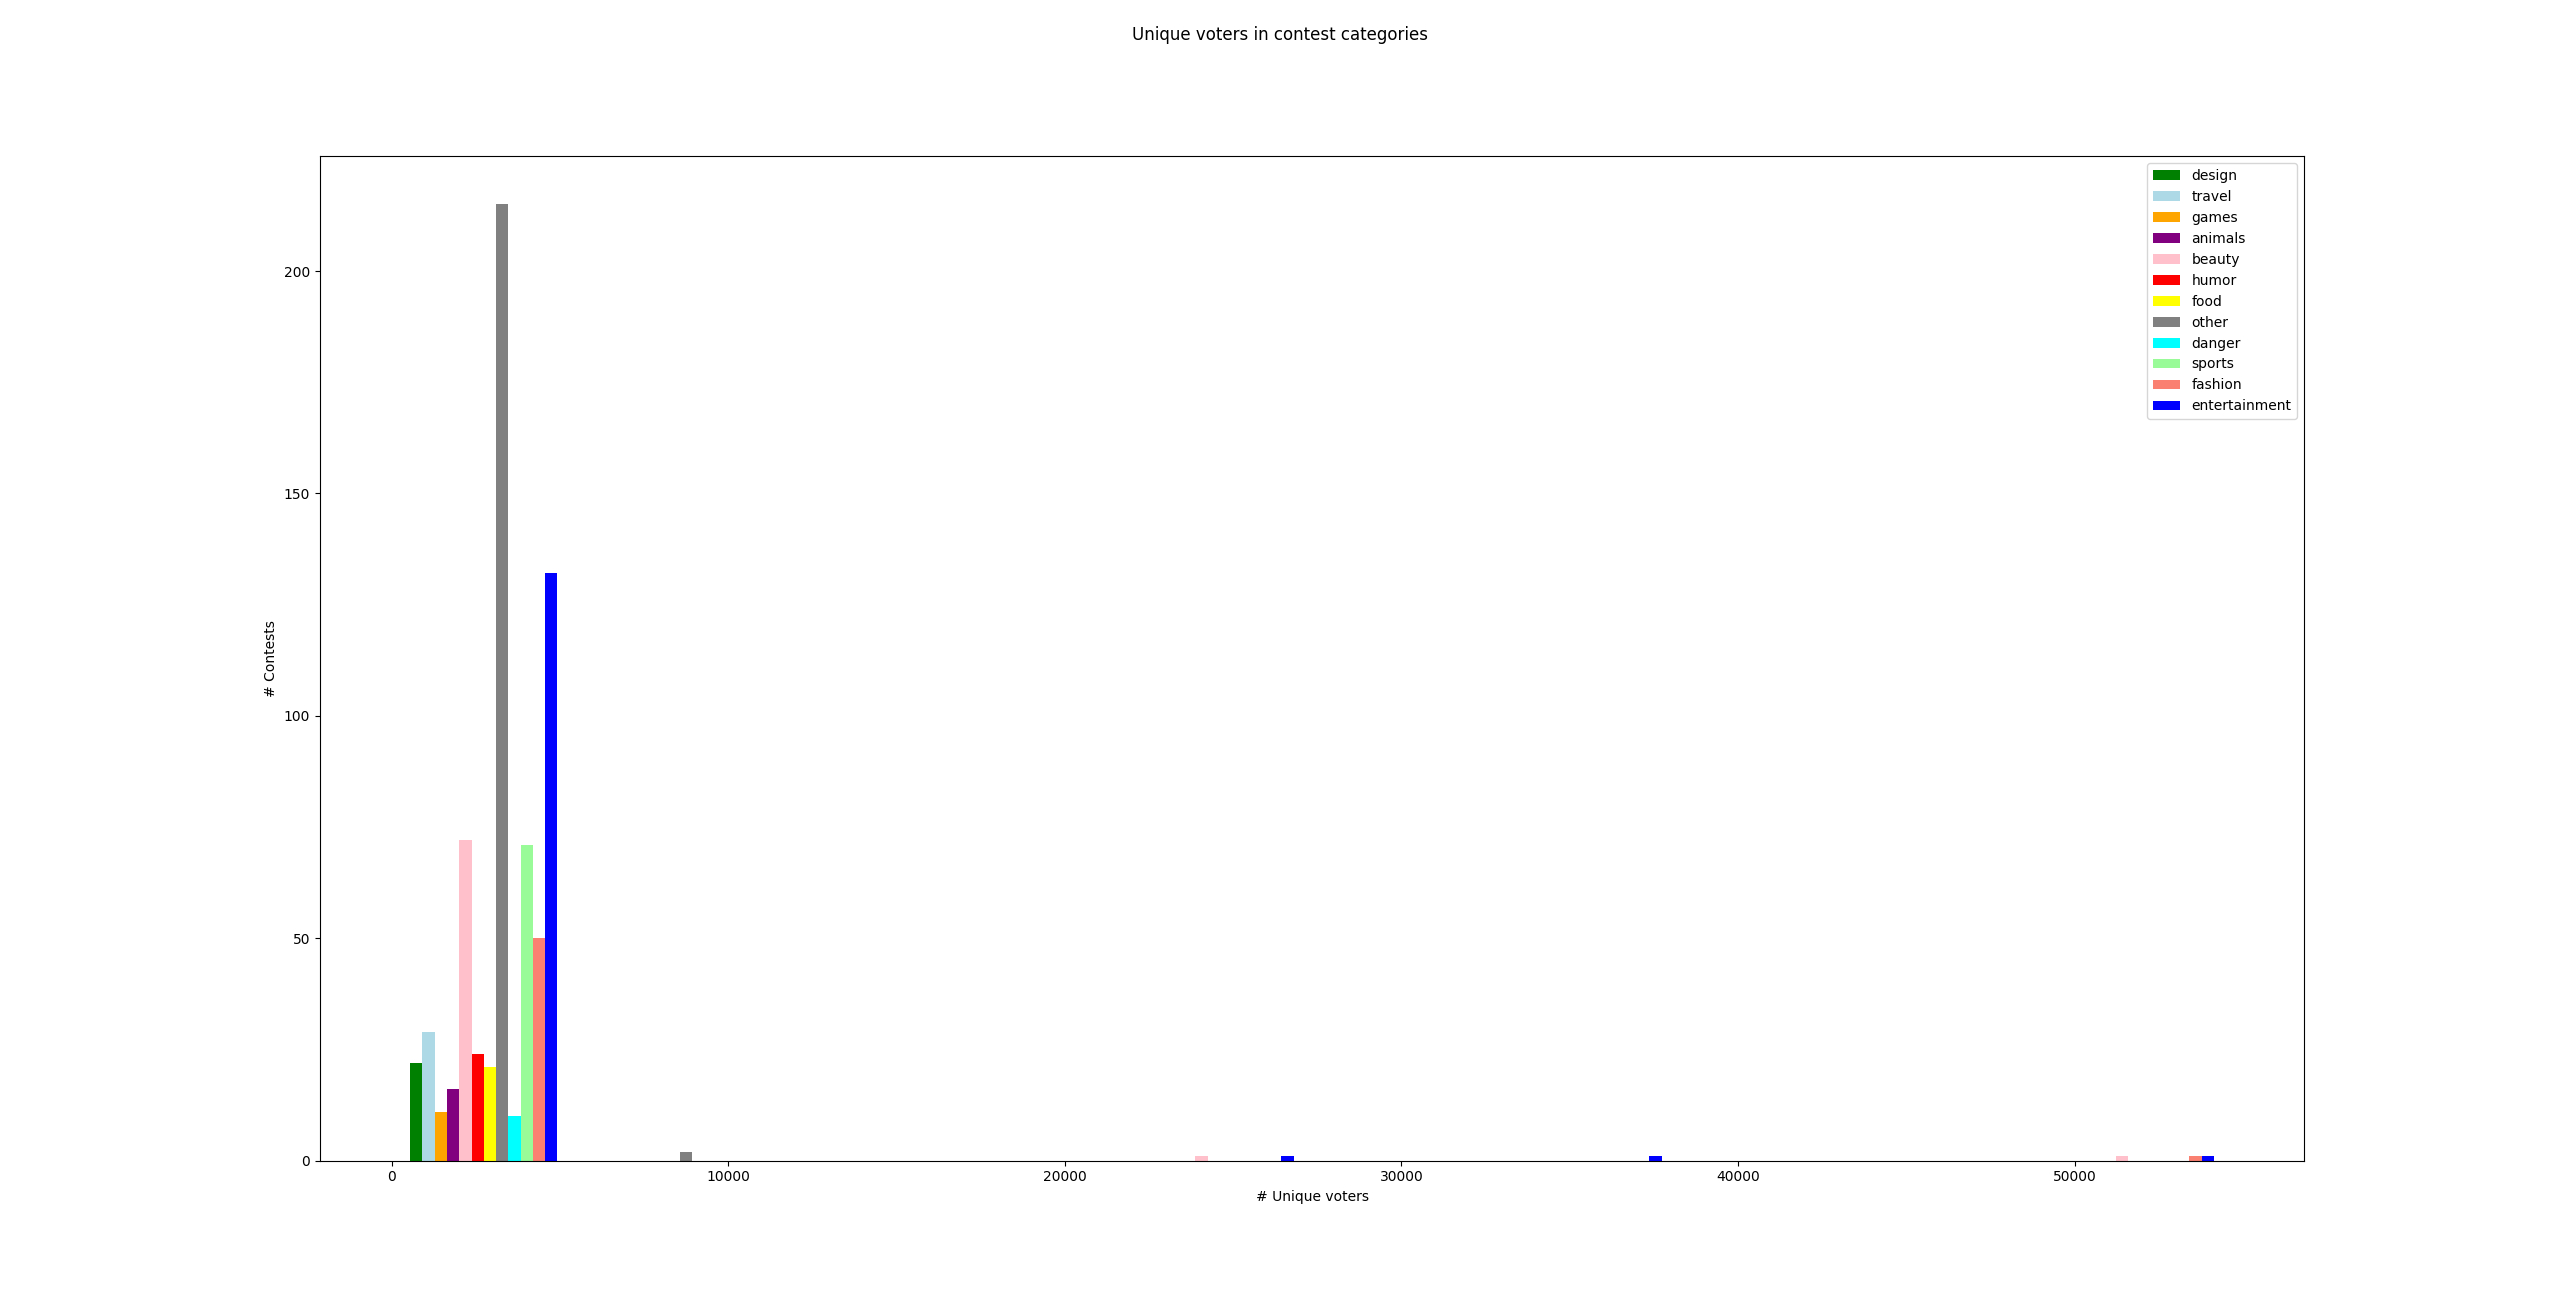
\includegraphics[width=0.8\textwidth]{Images/user_engagement_in_categories_bar.png}
                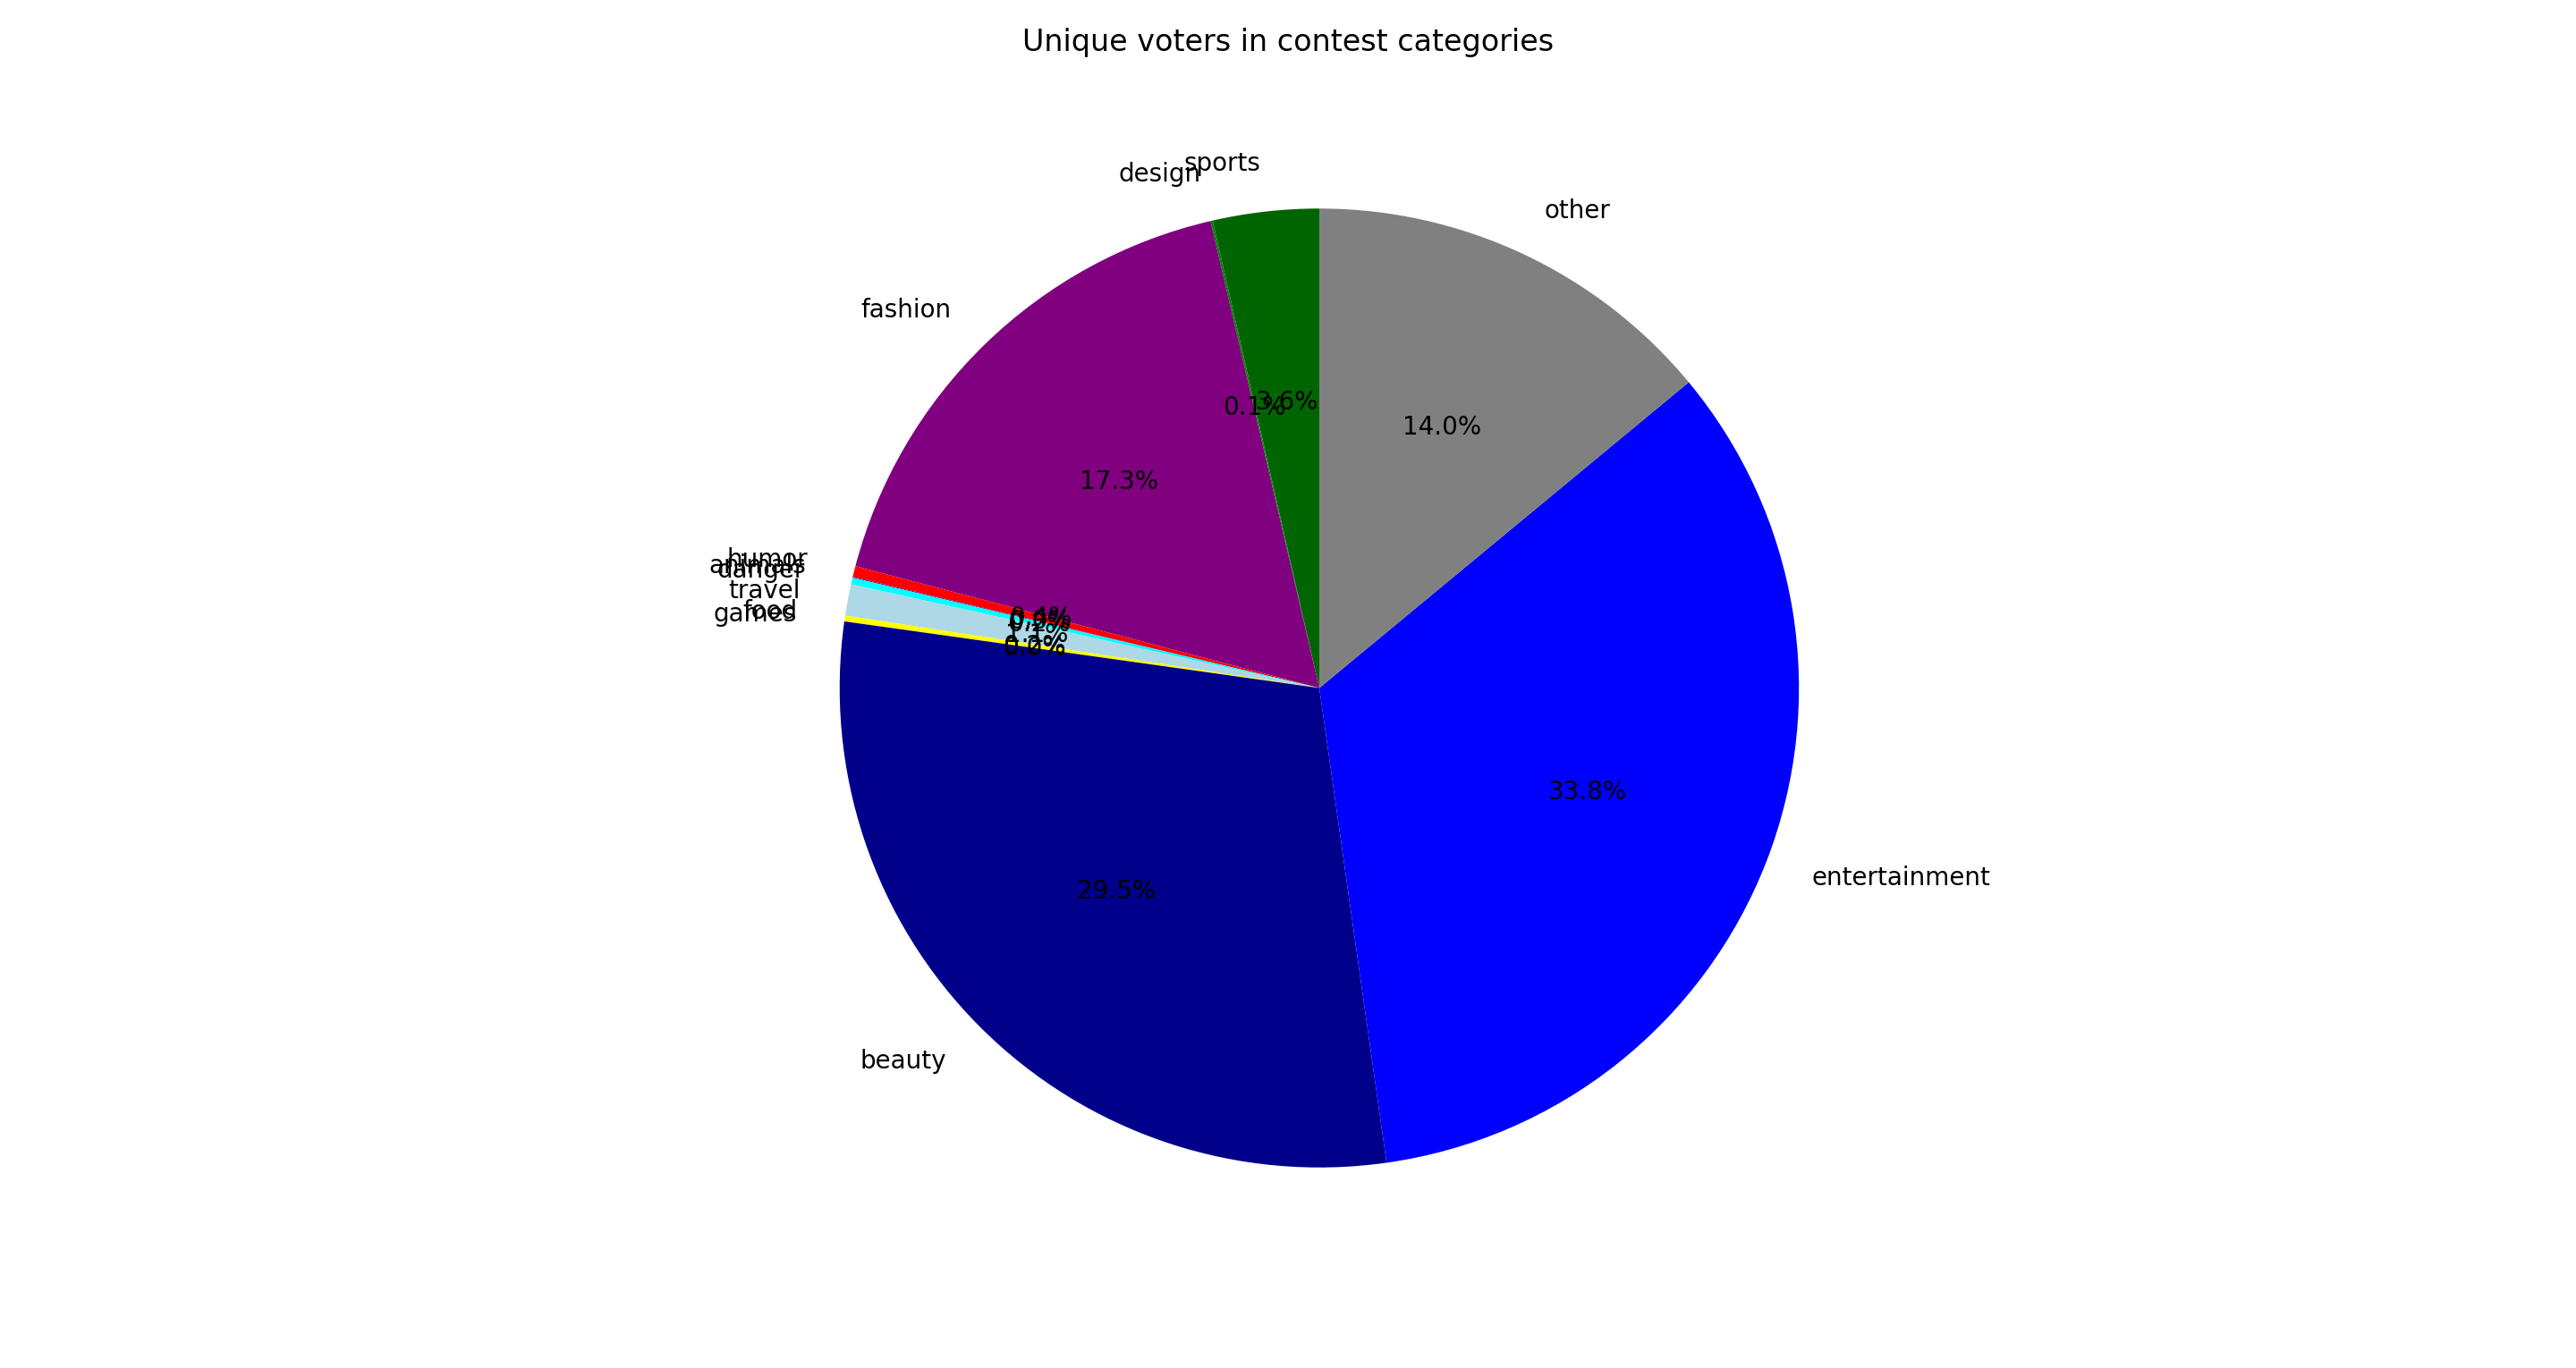
\includegraphics[width=0.8\textwidth]{Images/user_engagement_in_categories_pie.png}
                \caption{The number and percentage of unique voters over categories.}
                \label{user_engagement_in_categories}
            \end{center}
        \end{figure}
    
    % explain the distribution of users by gender, age group and country
    As the second part of EDA, the demographic data on user profiles was studied. Figure \ref{user_demographics_distribution} shows the distribution of 140 900 user profile in terms of gender, age group and country. This data is retrieved through each users profile, if they have given the related information or the privacy settings of the social media authentication allowed to retrieve the data. In case the information was not given or available from the social media profile, each filled was filled up with "other" values. It can be seen from the figure, that the distribution of males and females is considerably equal in the Choicely platform, but there is a large number of users, whose gender is unknown. Similarly, age group of users is often not known, however it can be seen that younger users are more active in Choicely, while elderly visitors are less engaged. 
    % TODO: explain nationalities as well in case anything interesting is gonna be done with them
    
    \begin{figure}[h] 
        \begin{center}
            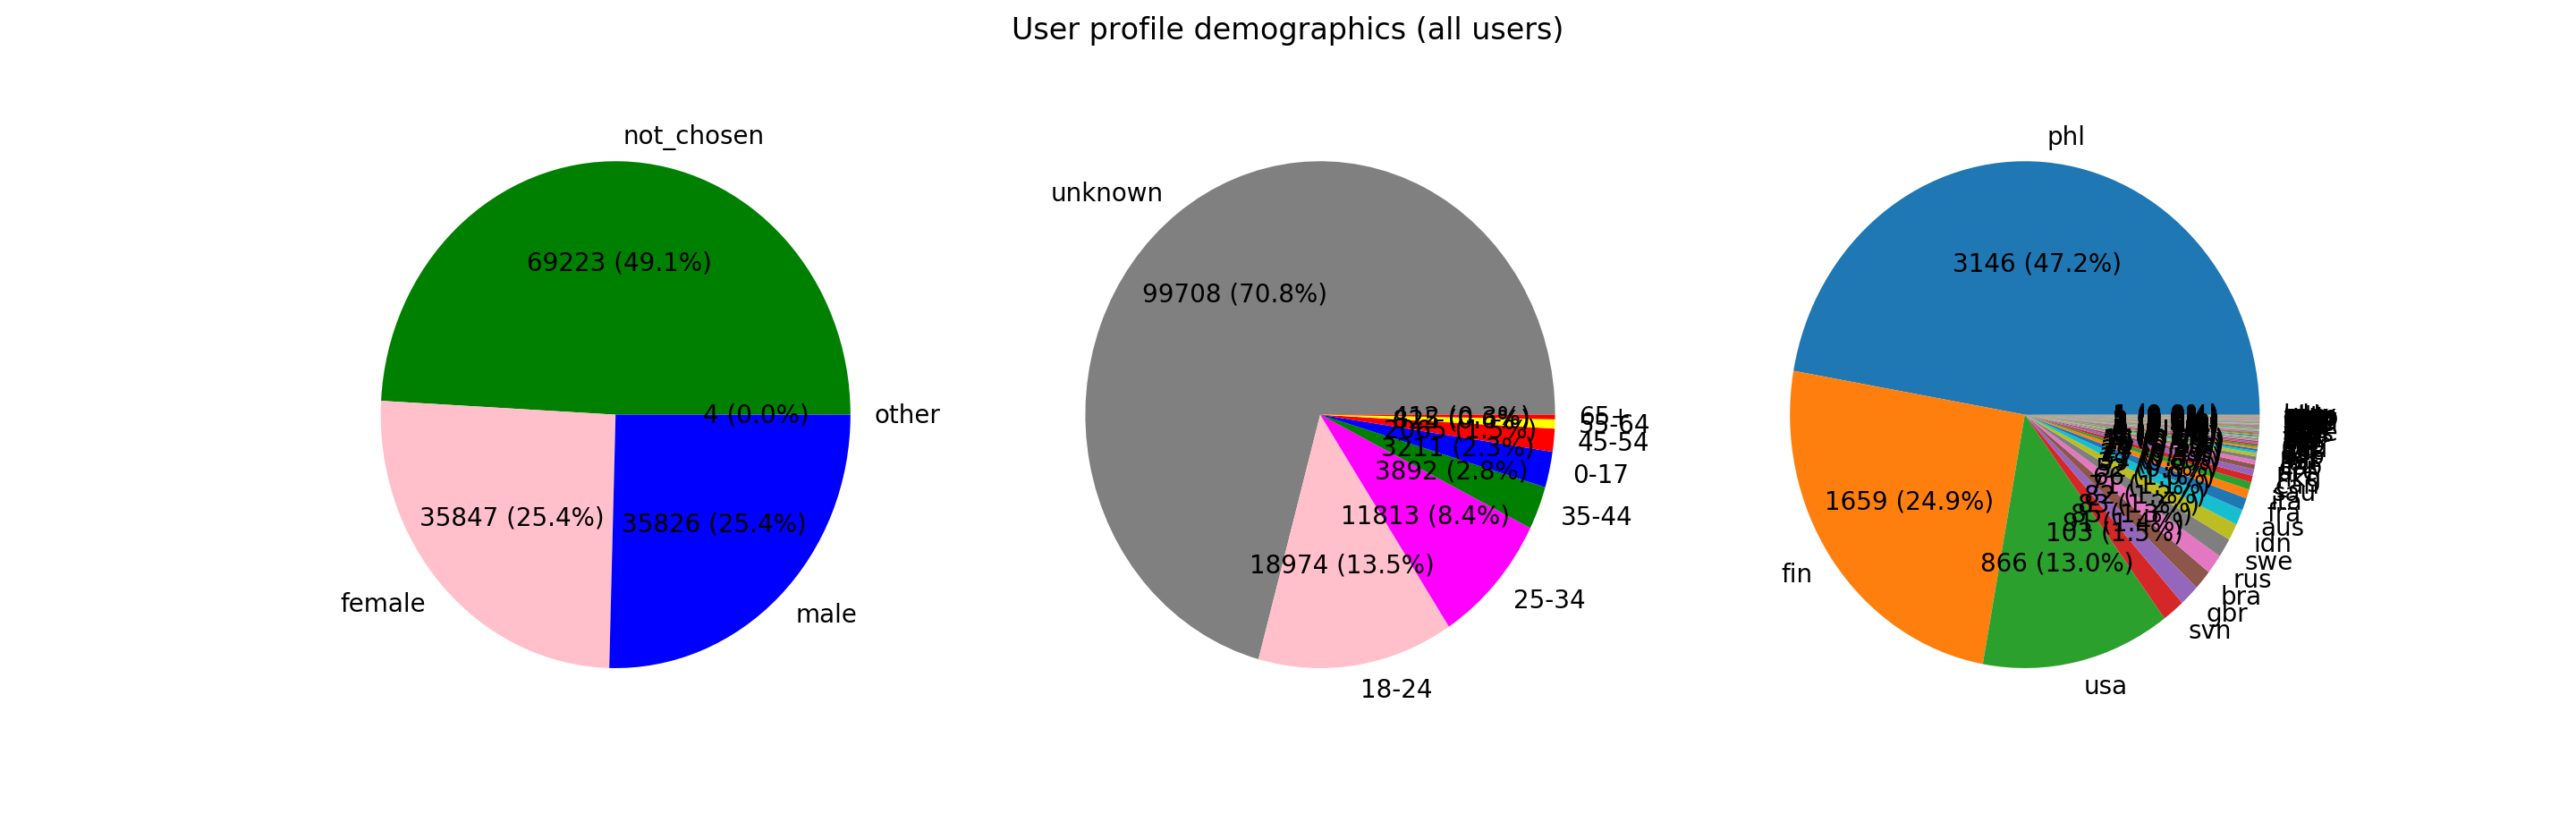
\includegraphics[width=0.8\textwidth]{Images/user_demographics_distribution.png}
            \caption{The distribution of demographic attributes over all users.}
            \label{user_demographics_distribution}
        \end{center}
    \end{figure}

    % compare to the distribution of users who have participated in more than 2 contest -> compare and elaborate   
    Thirdly, it was studied how often users return to participate in more than one contests. After retrieving all user profiles and their votes over all contests, the users who participated in less than 2 contests were filtered out. Figure \ref{user_demographics_distribution-pruned} displays the demographic attributes of such users. It can be seen that only a very small portion ($3362 / 140900 = 2.4 \% $) of the users return to participate in more than two contests. Interestingly however, $46.2 \%$ of the returning users are females, which is a big difference compared to their ratio in the overall population ($25.4 \% $, Figure \ref{user_demographics_distribution}). It allows the conclusion that females tend to be more active in terms of returning to vote in multiple contests. 

    \begin{figure}[h] 
        \begin{center}
            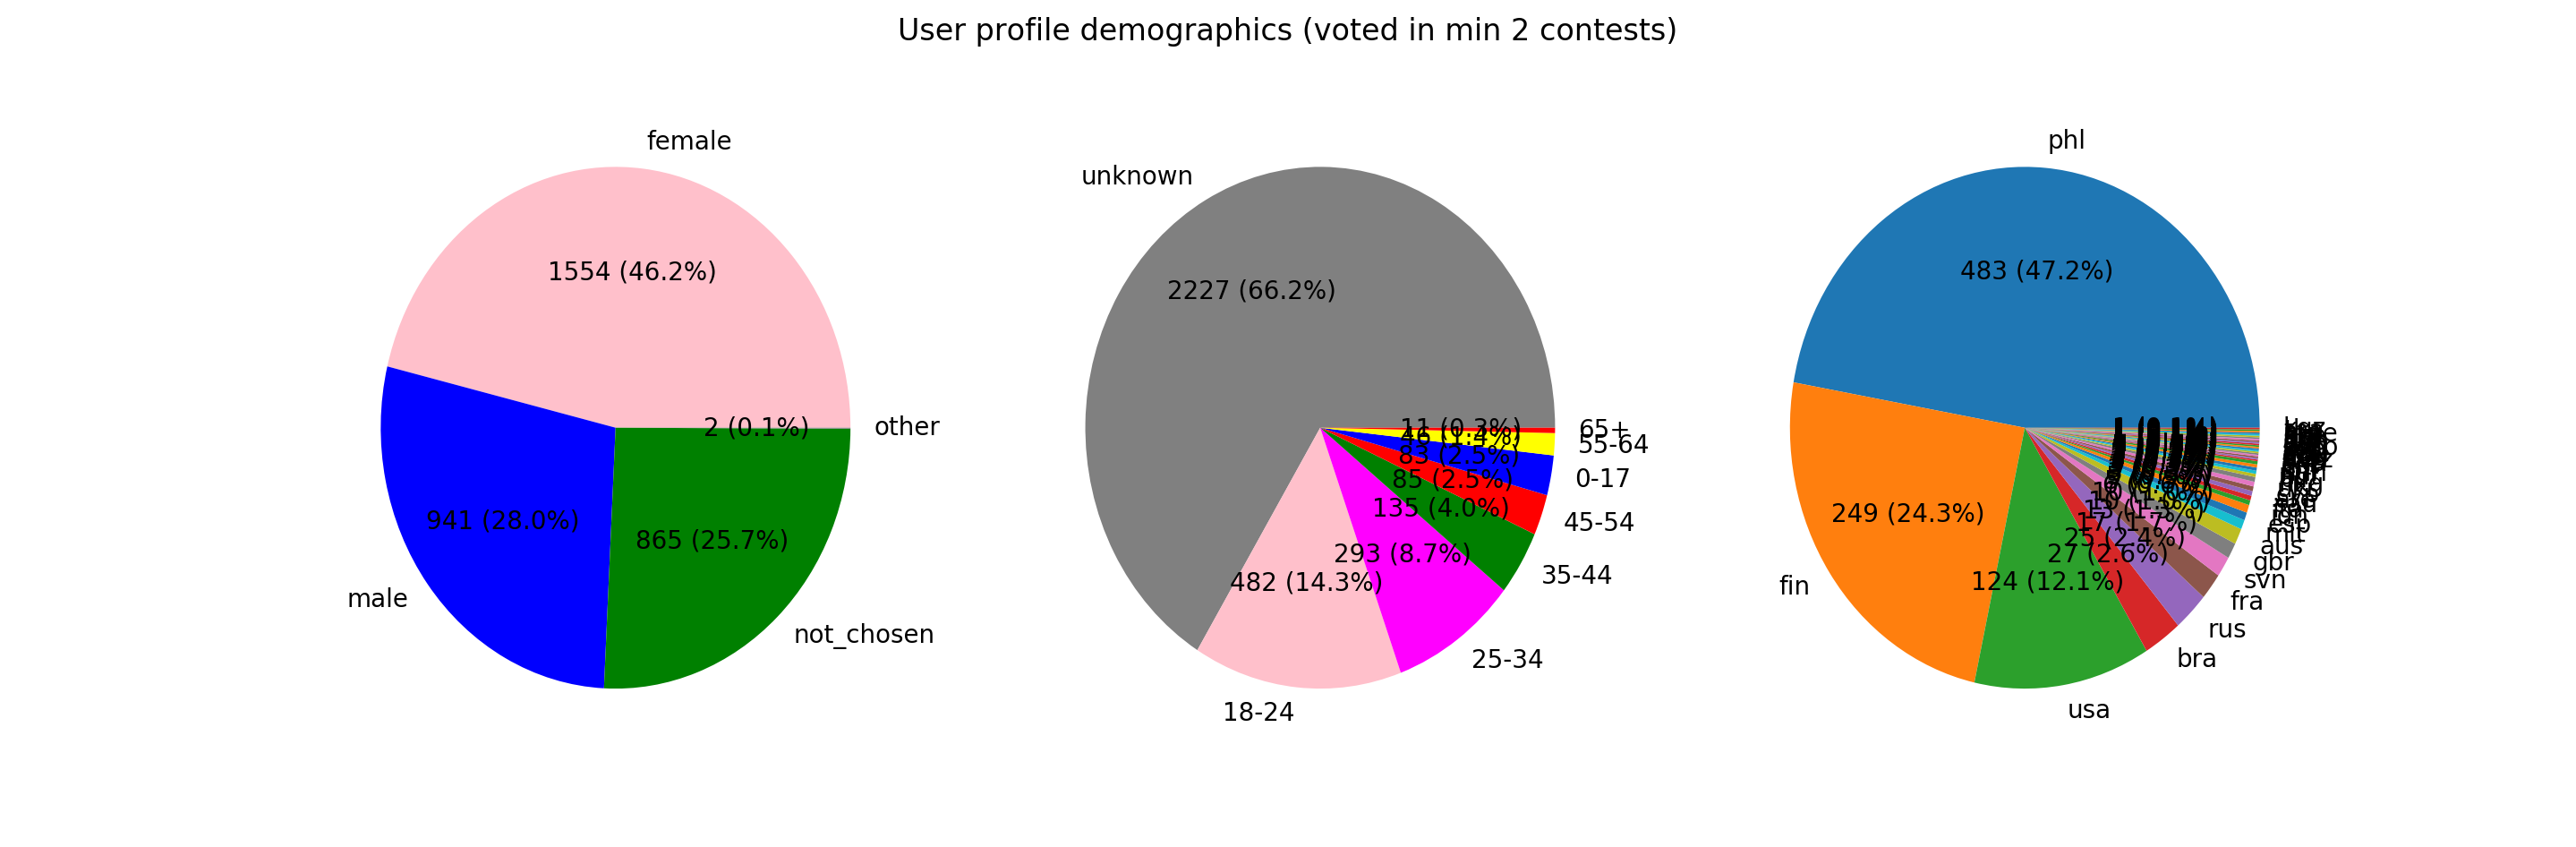
\includegraphics[width=0.8\textwidth]{Images/user_demographics_distribution-pruned}
            \caption{The distribution of demographic attributes over users who have participated in at least 2 contests.}
            \label{user_demographics_distribution-pruned}
        \end{center}
    \end{figure}

    % sum up and conclude
    The EDA has highlighted multiple ways how the data should be pruned in order to ensure the relevance of the data. (...)
    % TODO Conclusion

    \subsubsection{Preprocessing and pruning}
    It was identified, that some of the data cannot be used for the purposes of this study and the results will be more representative, if some of the data is pruned. Hence, the following rules were applied to prune the data:

    \begin {table}[]
        \centering
        \begin{tabular}{l|l}
            \textbf{Entity}              & \textbf{Pruning rule} \\
            \hline
            \textbf{Contest}             & Unique voters < 100 or Contest participants < 2
        \end{tabular}
        \caption{The pruning rules used for preprocessing the data.}
        \label{contest_preprocessing_rules}
    \end{table}

    % contests
    \begin{figure}[h] 
        \begin{center}
            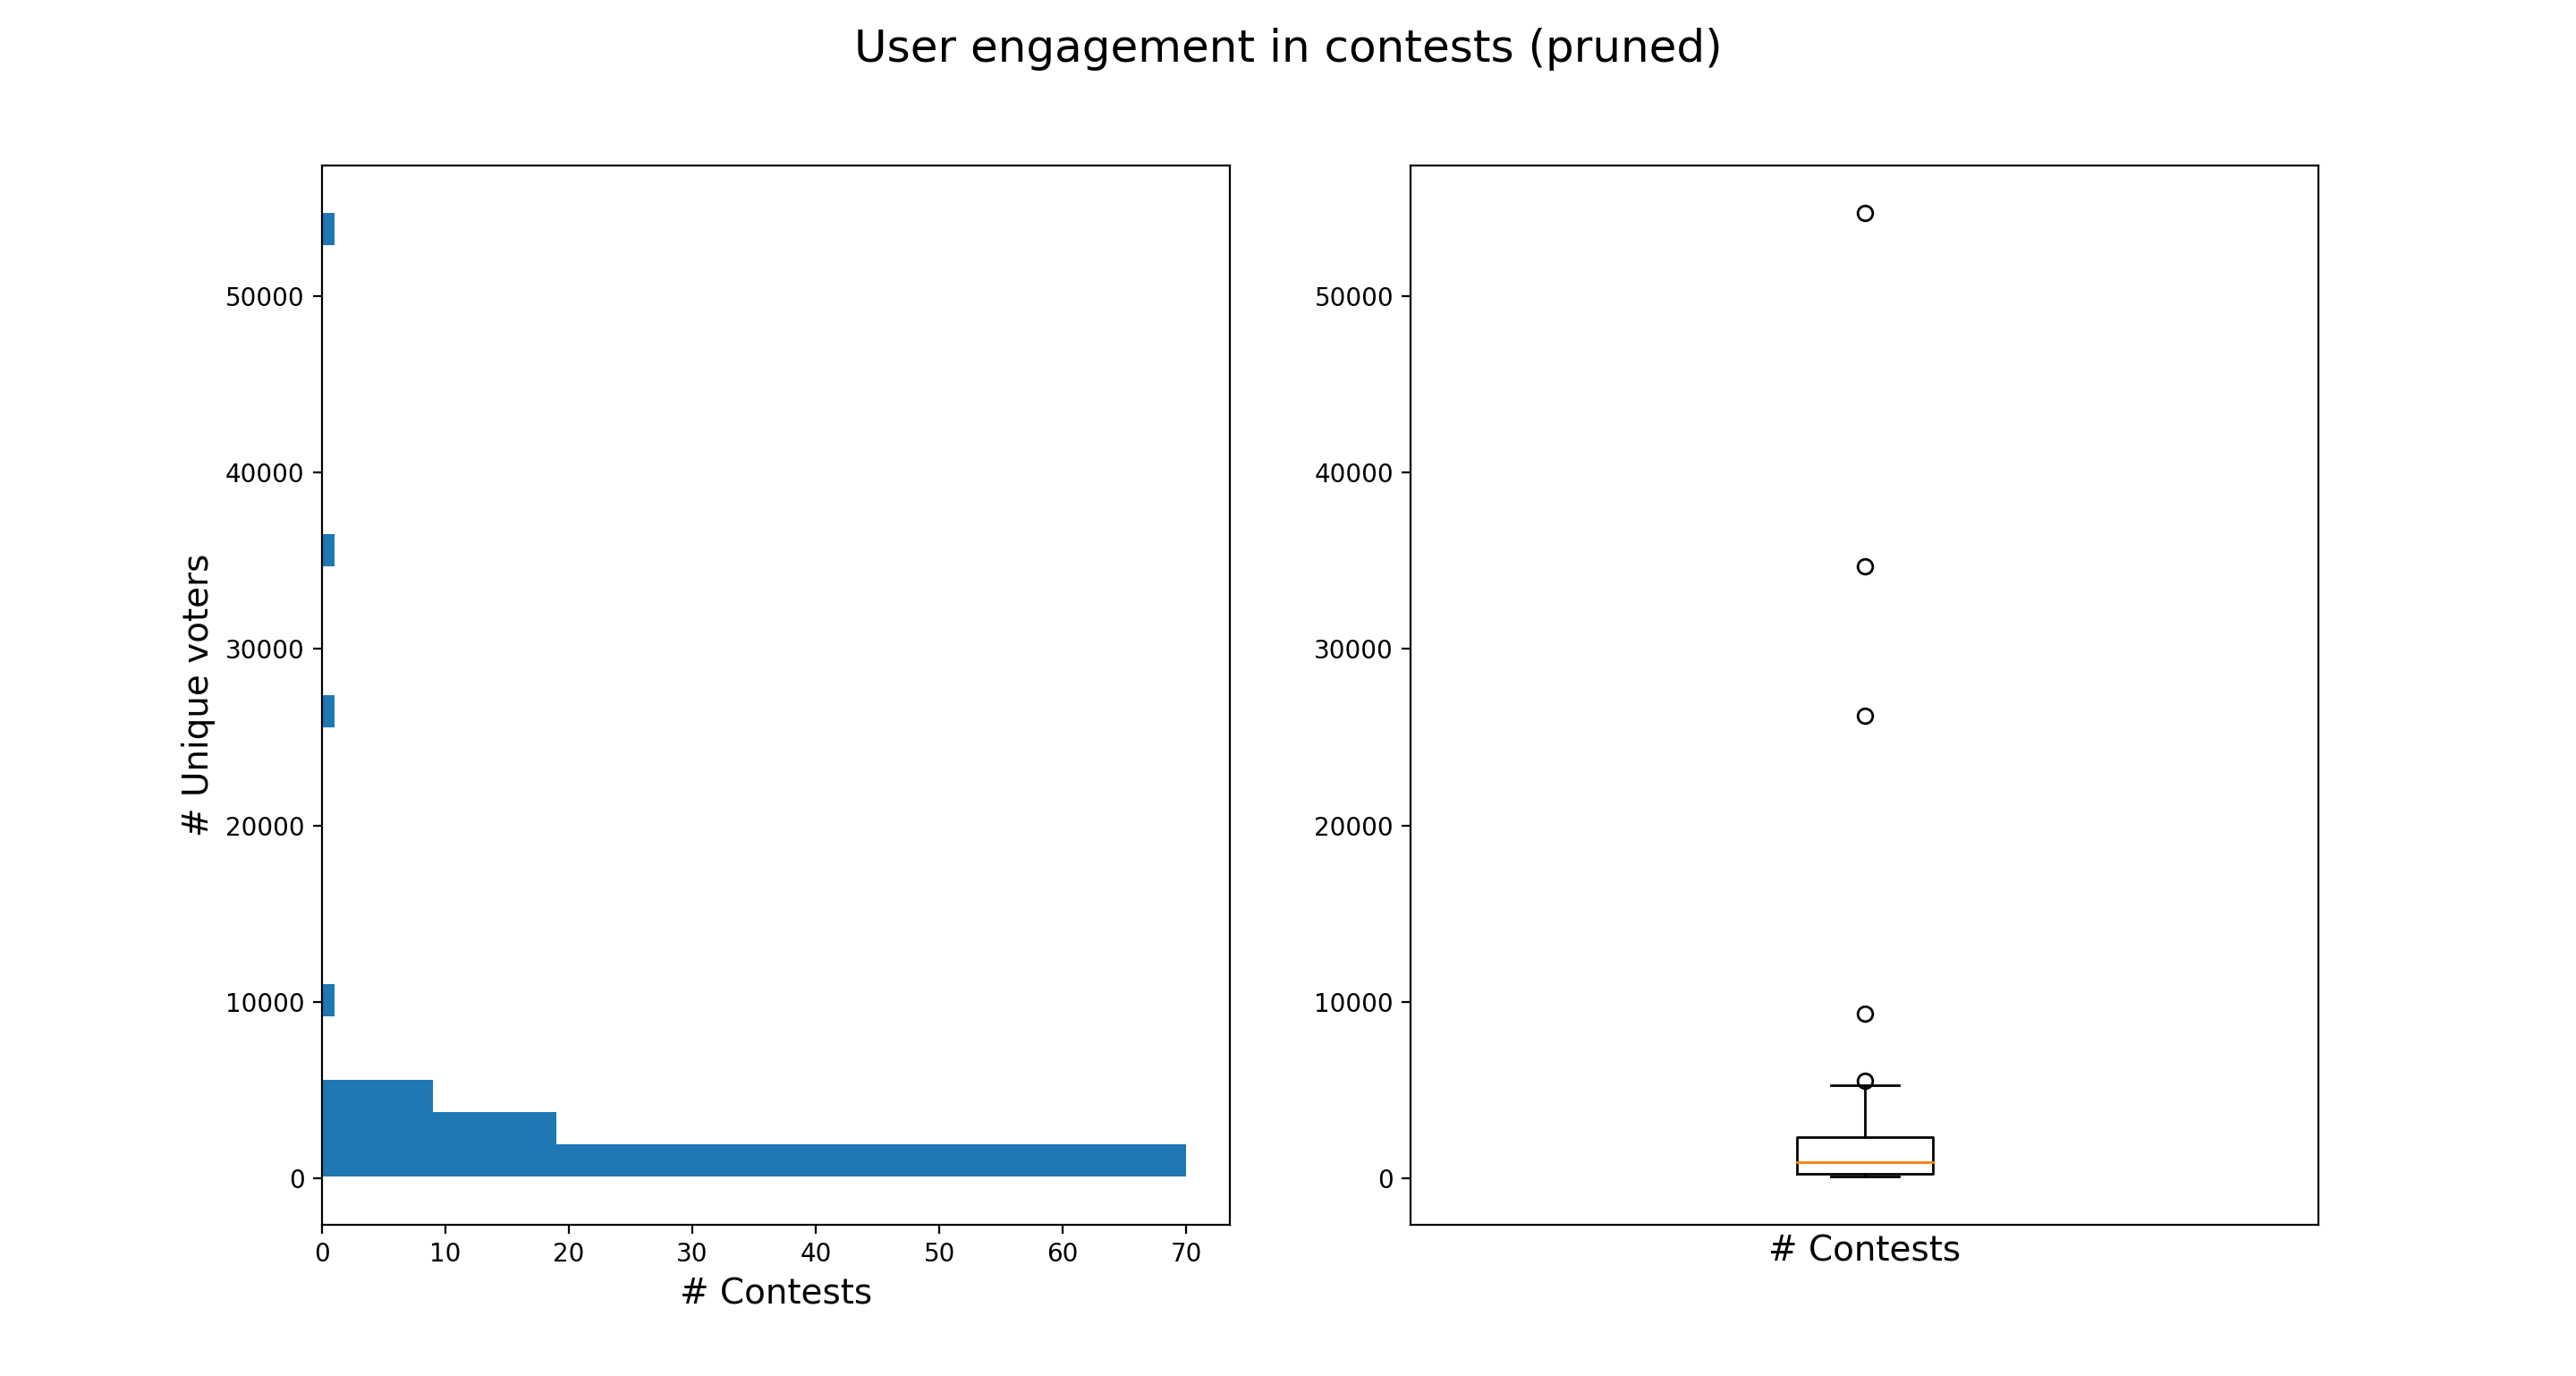
\includegraphics[width=0.8\textwidth]{Images/user_engagement_in_contests-pruned.png}
            \caption{}
            \label{}
        \end{center}
    \end{figure}

    \begin{figure}[h] 
        \begin{center}
            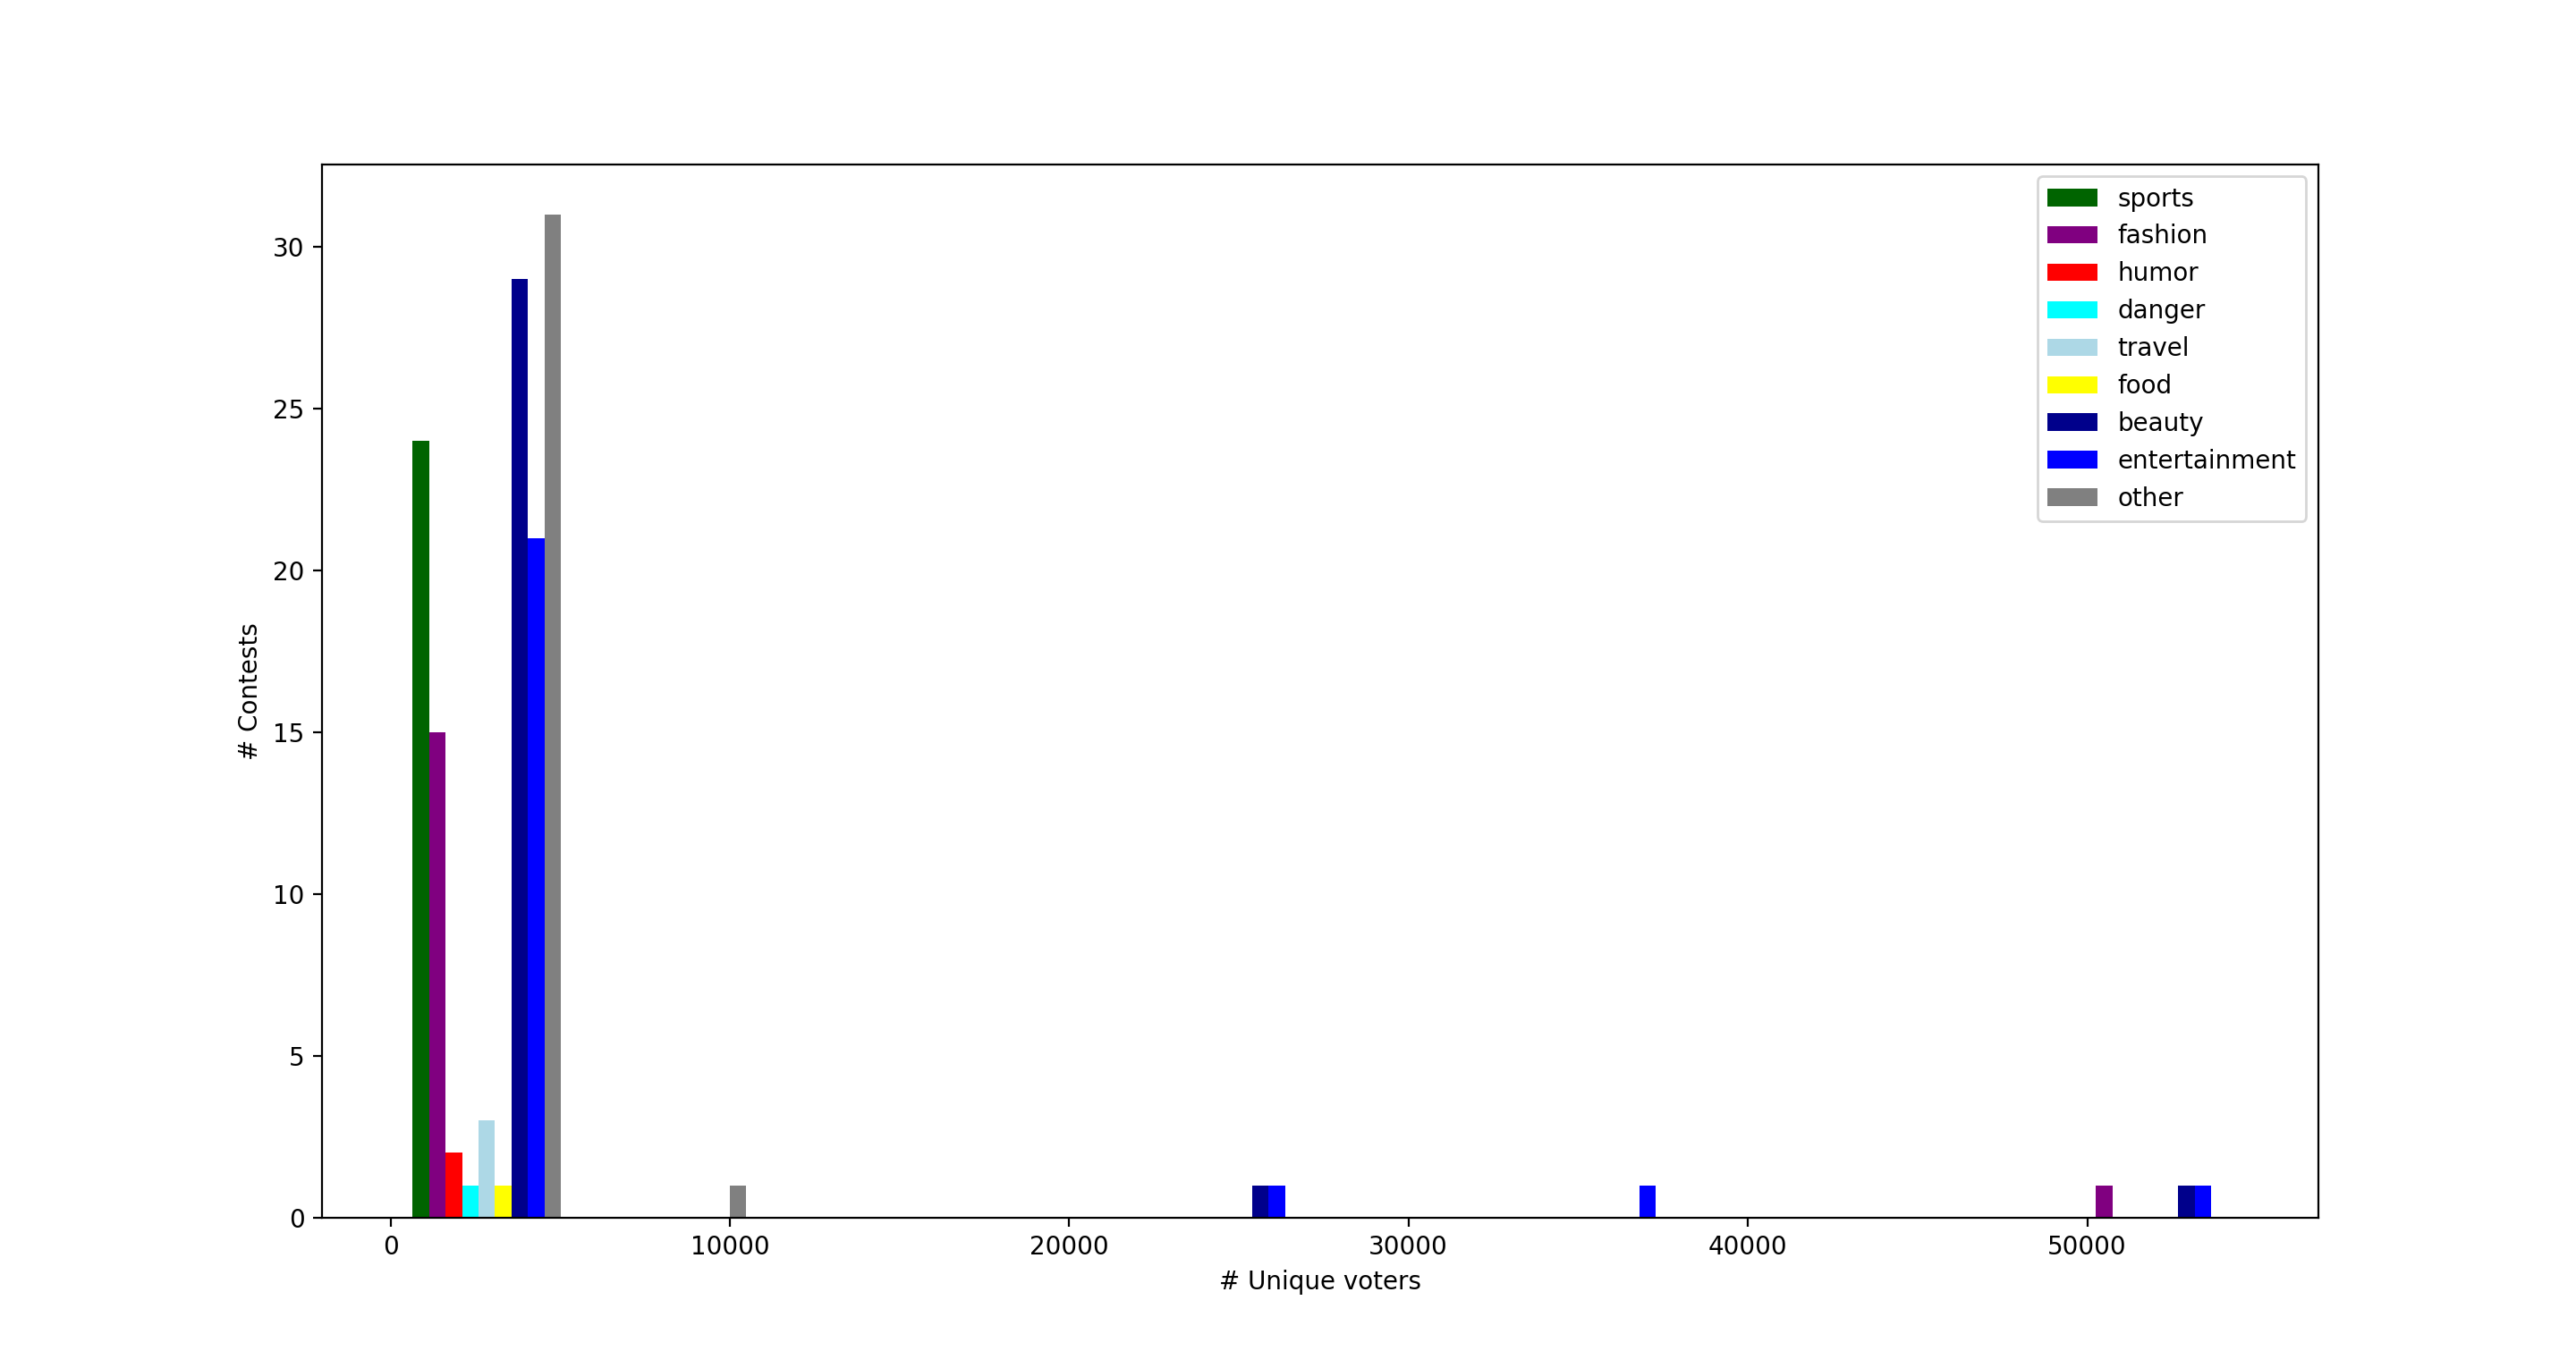
\includegraphics[width=0.8\textwidth]{Images/user_engagement_in_categories_bar-pruned.png}
            \caption{}
            \label{}
        \end{center}
    \end{figure}
    
    \begin{figure}[h] 
        \begin{center}
            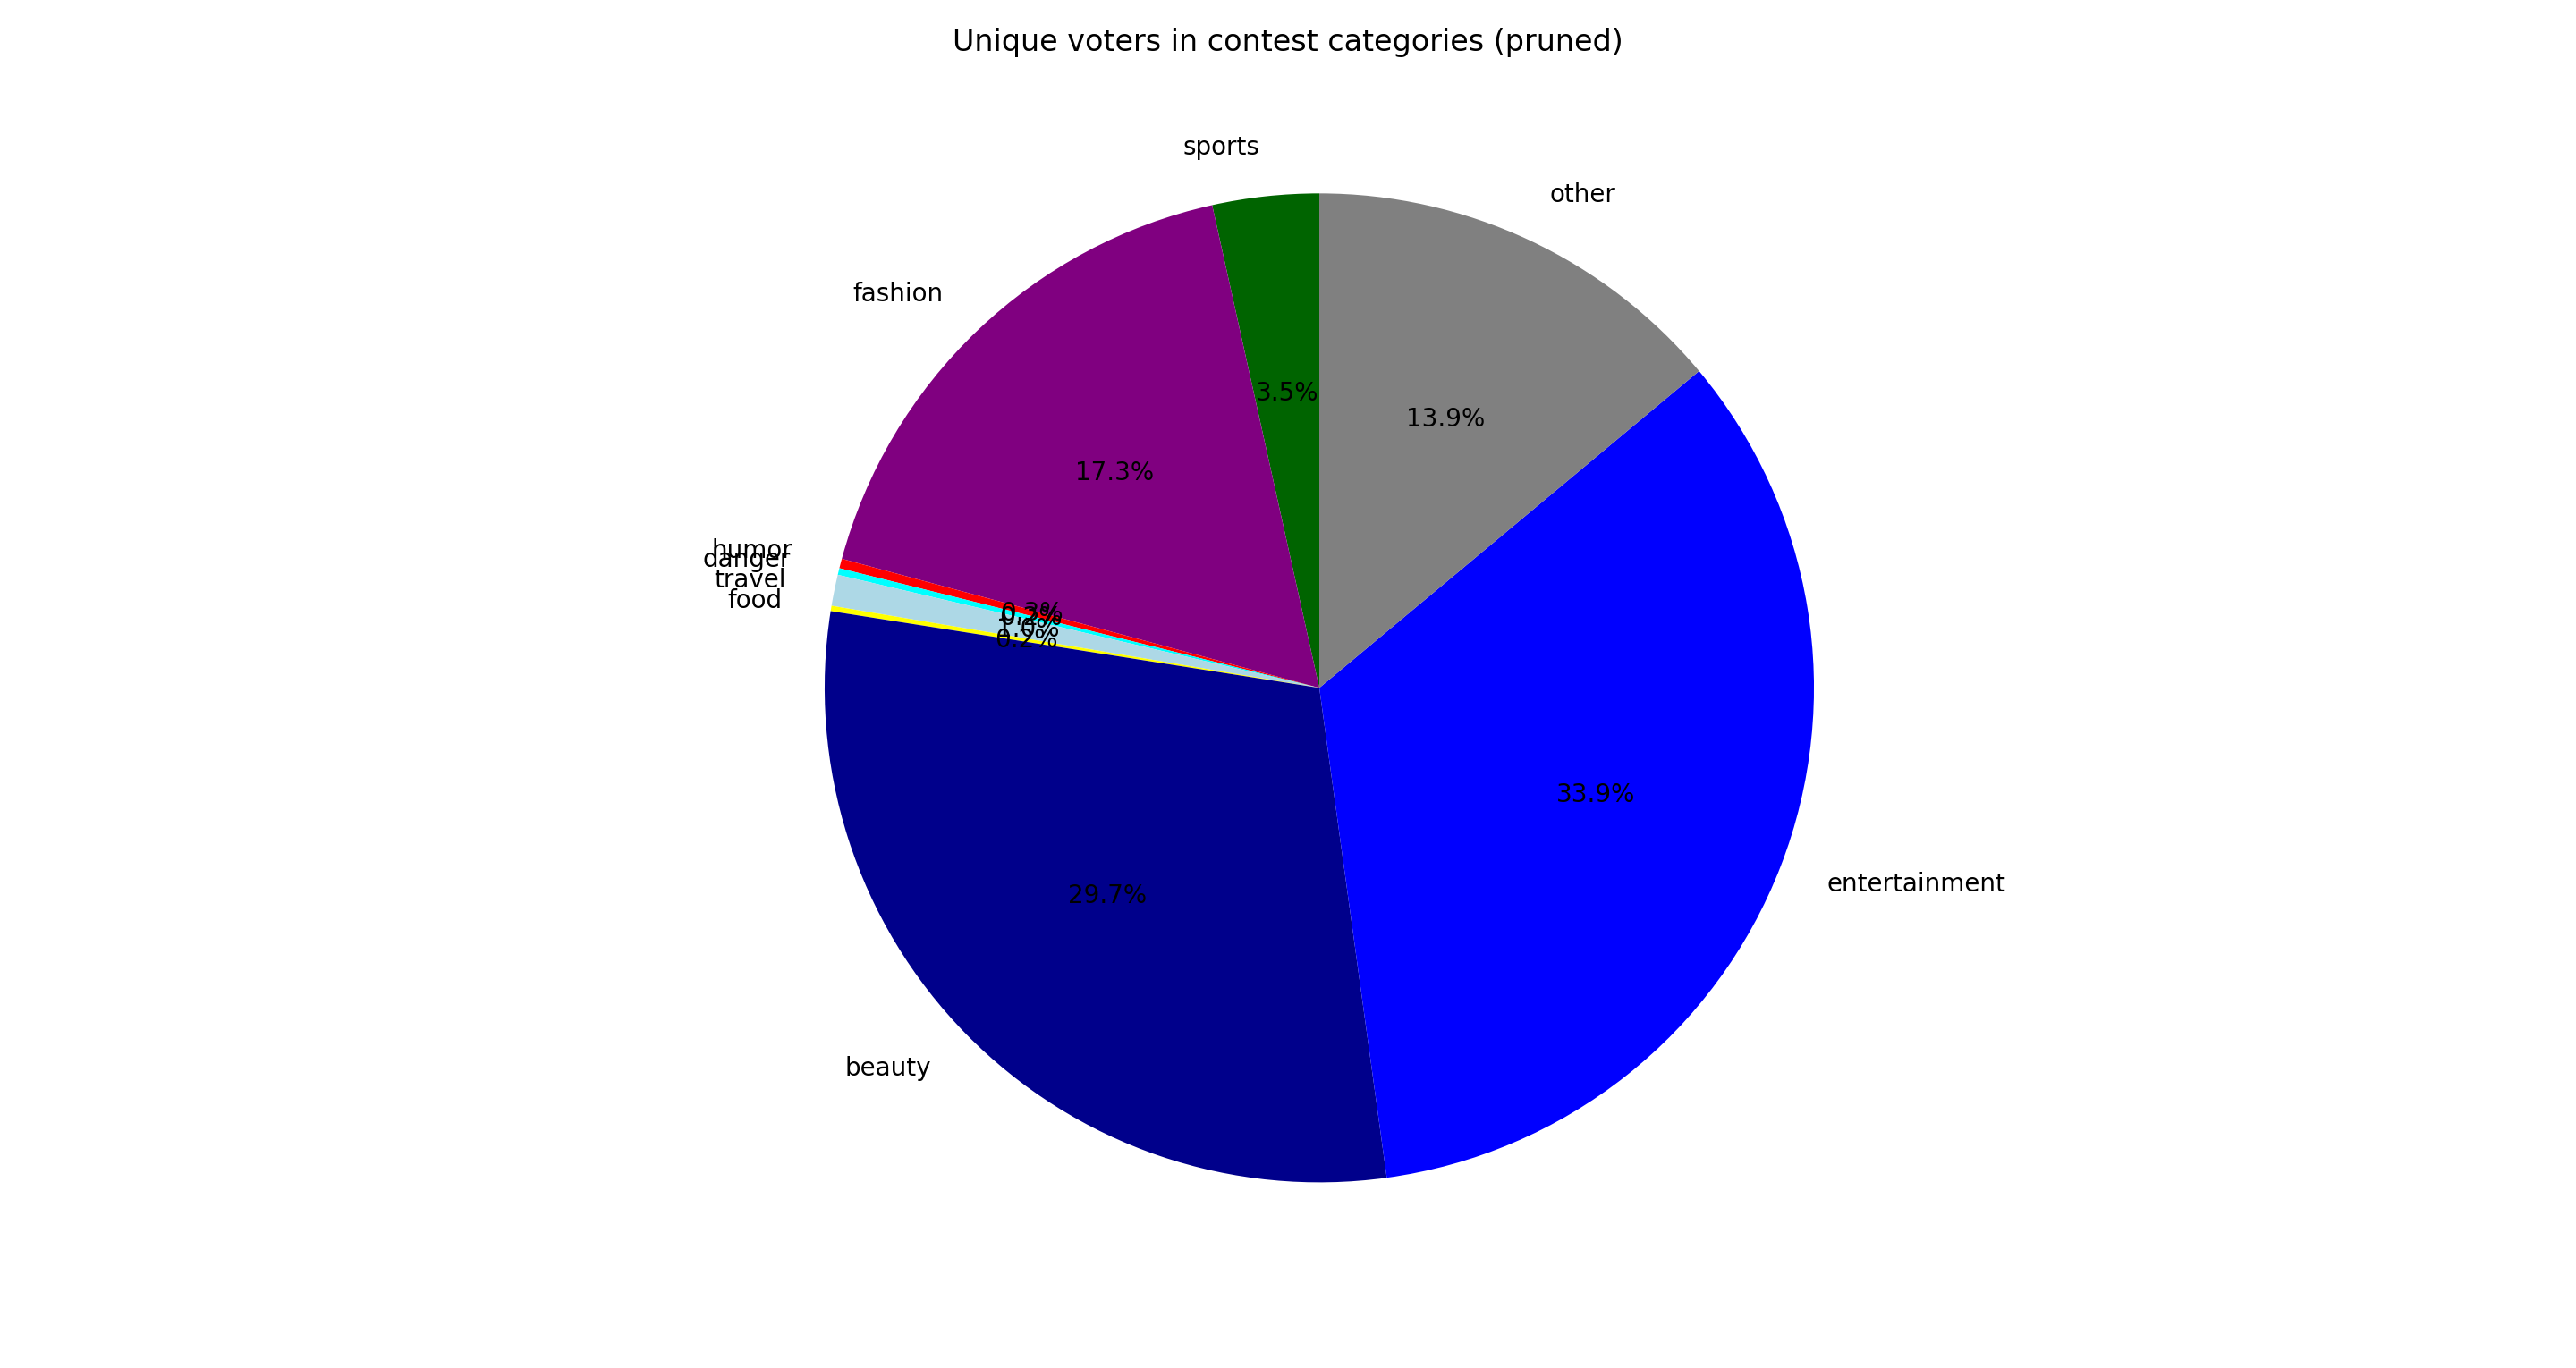
\includegraphics[width=0.8\textwidth]{Images/user_engagement_in_categories_pie-pruned.png}
            \caption{}
            \label{}
        \end{center}
    \end{figure}
    % users

    % Entities that match any of the rules displayed in Table \ref{preprocessing_rules} are dropped from the analysis. For instance, contests with less than 100 unique voters (users) and images without labels are considered irrelevant, and may bias the results of the study. After applying the preprocessing rules, the dataset is left with 92 contests, 1625 contest participants, 282545 votes and XXX unique voters over 10 contest categories. % TODO update occasionally

    \subsubsection{Association analysis}
    Some initial results for the Miss Fitness Finland contest \footnote{\url{https://choicely.com/contests/7a7b90f8-84c7-11e7-a452-a9f8b94782fe}}: 

    [jewellery]
    Male ----------------------------------------------------------------------------------------------------o------------0.13--------------------------------------------------------------------------------------- Female
    
    [jewellery, beauty]
    Male ----------------------------------------------------------------------------------------------------o------------0.13--------------------------------------------------------------------------------------- Female

    [jewellery, human hair color]
    Male ----------------------------------------------------------------------------------------------------o------------0.13--------------------------------------------------------------------------------------- Female
    
    [shoulder, beauty, hair]
    Male ----------------------------------------------------------------------------------0.18-----------------o---------------------------------------------------------------------------------------------------- Female

    [model, shoulder, hair]
    Male ----------------------------------------------------------------------------------0.18-----------------o---------------------------------------------------------------------------------------------------- Female
    [human hair color, shoulder, hair]
    Male ----------------------------------------------------------------------------------0.18-----------------o---------------------------------------------------------------------------------------------------- Female
        

    \begin{figure}[h] 
        \begin{center}
            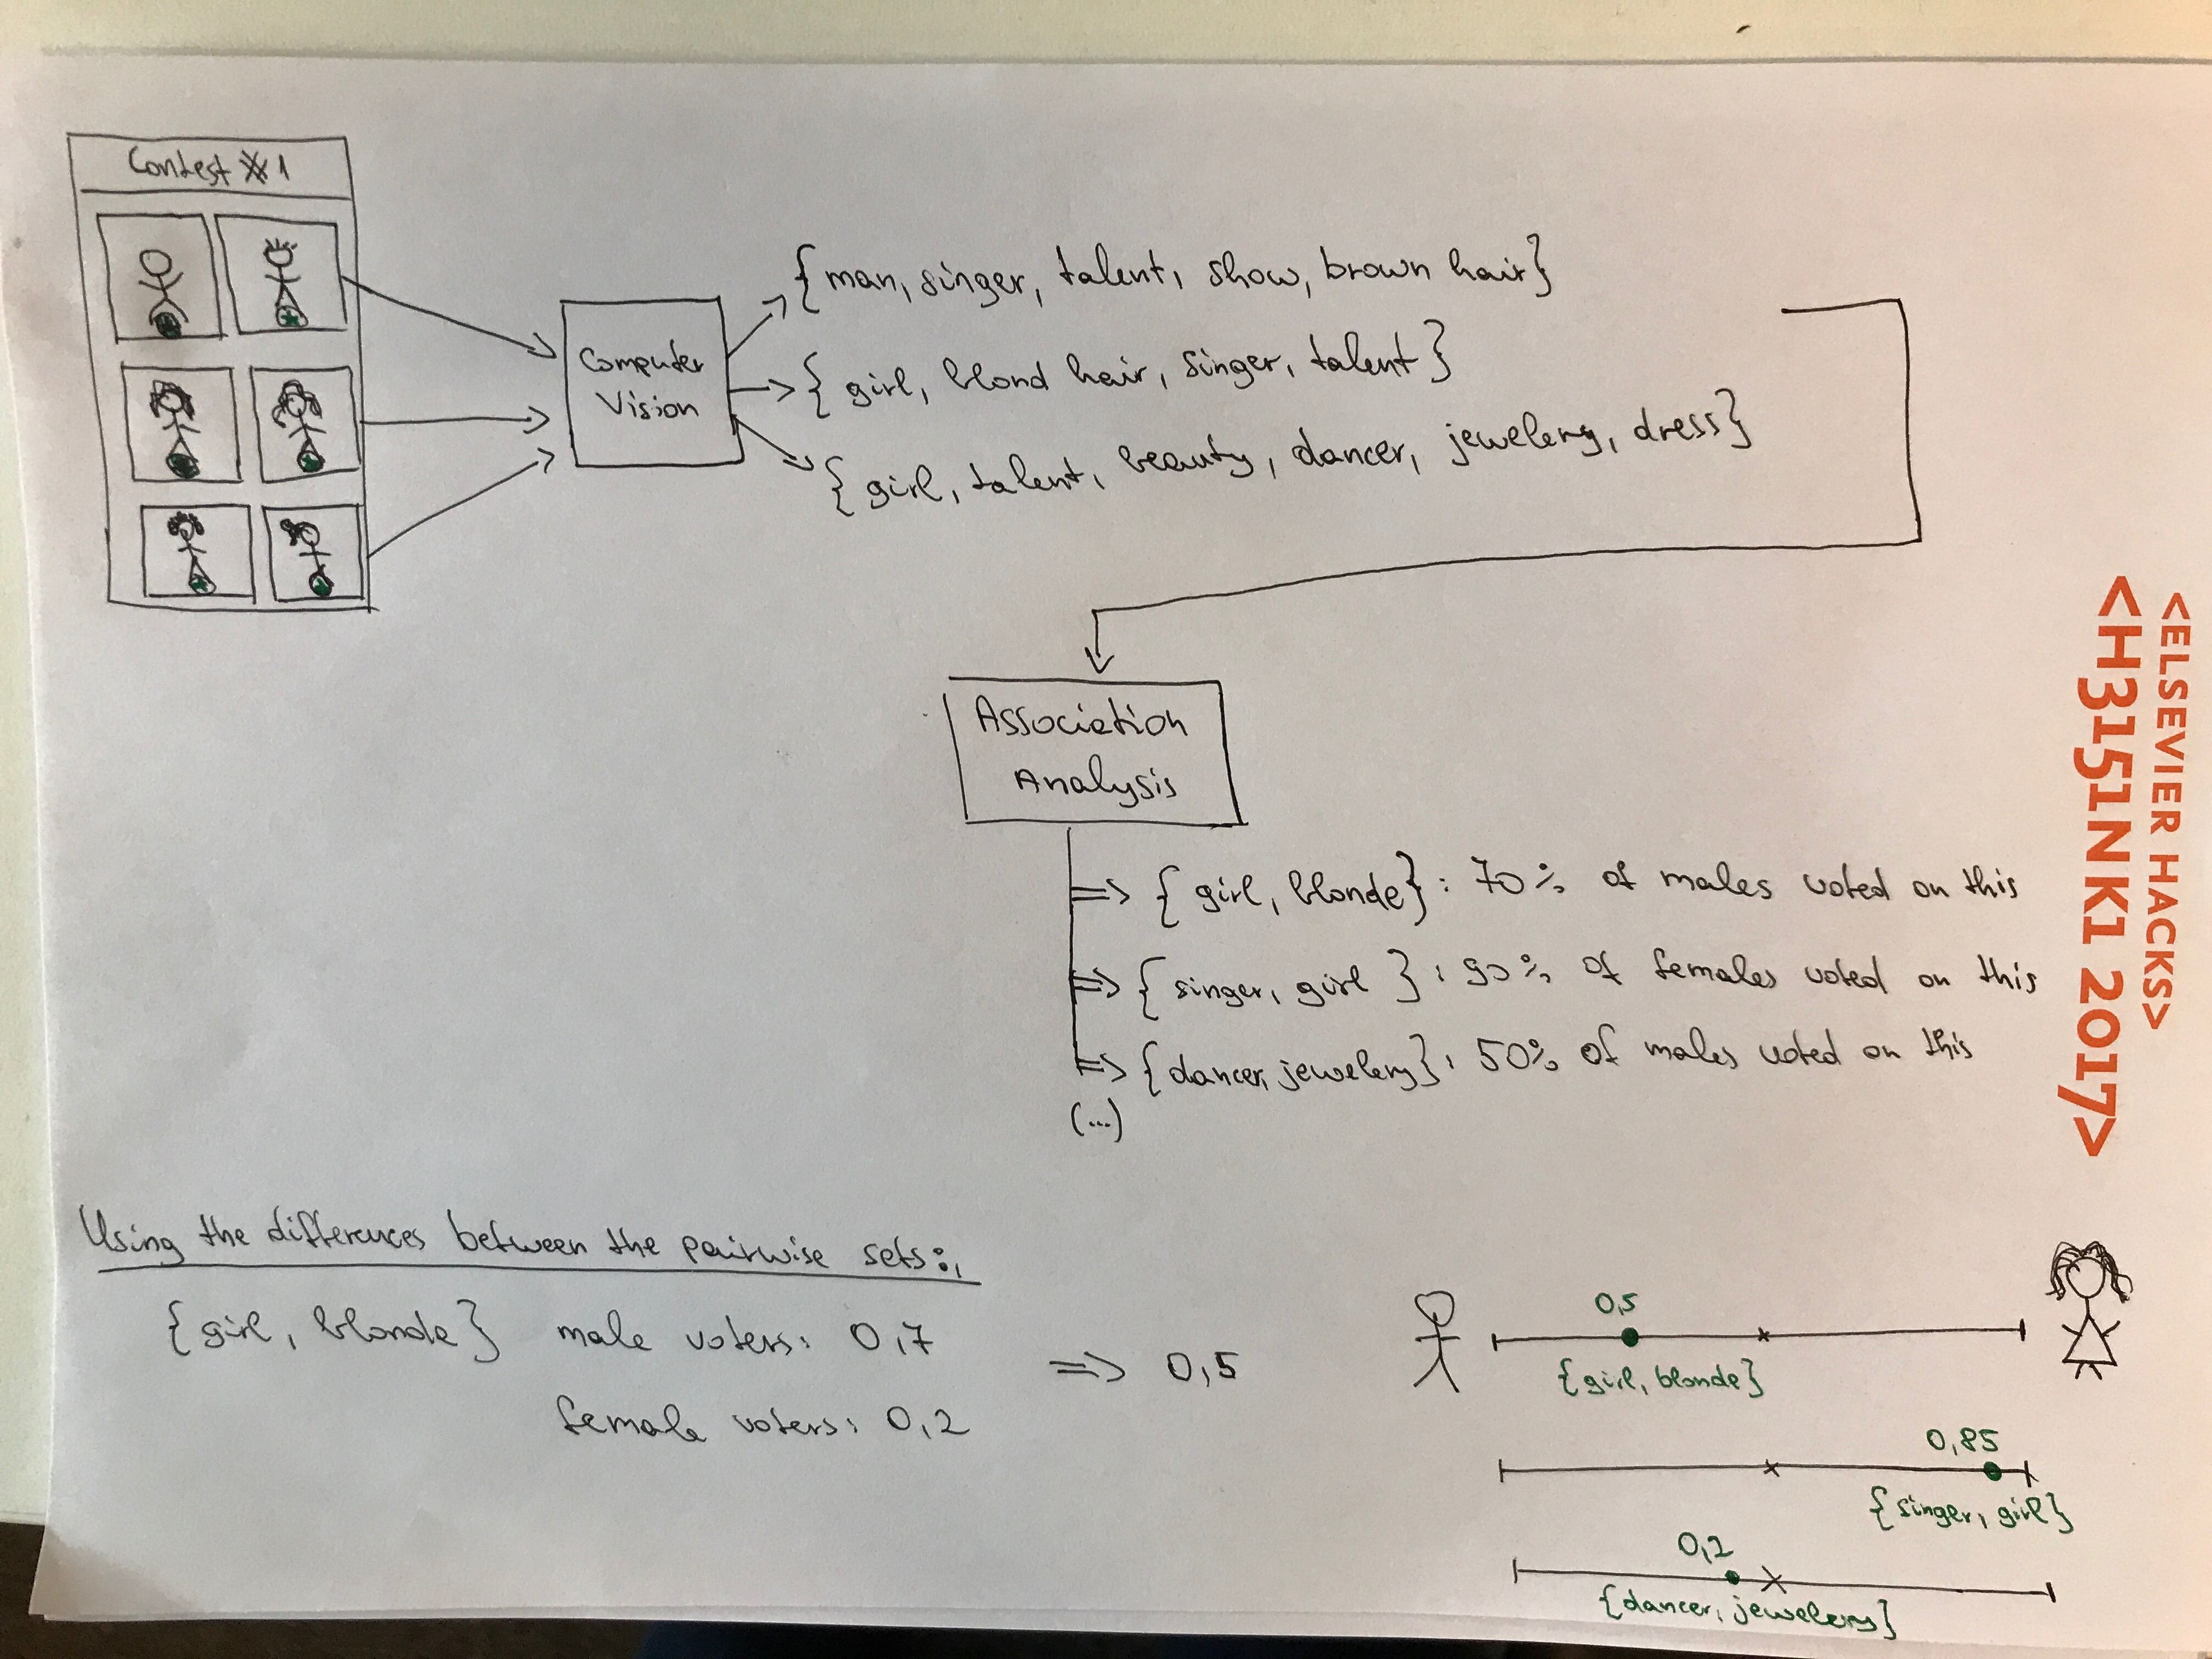
\includegraphics[width=0.8\textwidth]{Images/association_analysis_flow.jpg}
            \caption{The flow of the association analysis of the participants' images.}
            \label{association_analysis_flow}
        \end{center}
    \end{figure}

